\cleardoublepage\documentclass[../main.tex]{subfiles}
\begin{document}
\chapter{A Integral Indefinida}\label{cap:IntIndefinida}
\minitoc
%\tableofcontents
\subsection*{Objetivos de aprendizagem do capítulo}
\addcontentsline{toc}{section}{Objetivos de aprendizagem do capítulo}
\noindent Ao final deste capítulo você deverá ser capaz de:
\begin{itemize}
    \item Compreender o significado da integral indefinida;
    \item  Familiarizar-se com as fórmulas básicas de integração;
    \item Aplicar corretamente os métodos de integração;
    \item  Determinar as integrais de funções racionais e irracionais.
\end{itemize}

\section{Introdução}
No estudo da derivada, o problema básico da derivação é: dado o recorrido de um ponto móvel, calcular sua velocidade, ou dada uma curva, calcular sua inclinação, isto é, obter, a partir de uma função, outra função chamada de derivada.

Neste capítulo, o problema básico da integração é o caso inverso da derivação: dada a velocidade de um ponto móvel em cada instante, encontrar sua trajetória, ou dada a inclinação de uma curva em cada um de seus pontos, calcular a curva, ou seja, encontraremos ou determinaremos uma função original que chamaremos de antiderivada. Por tal motivo, aprenderemos algumas das técnicas para encontrar as antiderivadas aplicando as regras de derivação estudadas no Capítulo \nameref{chap:derivadas}.
\section{A Antiderivada}\label{Cap:IntInd-sec:Antiderivada}
Estudar o cálculo diferencial trata-se, principalmente, de: dada uma função, encontrar sua derivada. No entanto, muitas aplicações importantes do cálculo têm uma relação com o problema inverso, isto é: ``dada uma função \(f\) definida em um intervalo \(I\), encontrar uma função \(F\) cuja derivada seja a função \(f\), ou seja, \(F'(x)=f(x)\) para cada \(x\) pertencente ao intervalo \(I\)''.

Mais formalmente, temos a seguinte definição.

\begin{framed}
\begin{definition}\label{def:DefAntiderivada}
Diz-se que a função \(F\) é uma antiderivada da função \(f\) no intervalo \(I\), se

\[ F'(x)=f(x), \quad \forall\,x\in I. \]
\end{definition}
\end{framed}

\begin{ex}
Sejam as funções \(f(x)=4x^3\) e \(g(x)=e^{x}\), com \(x\in \mathbb{R}\). Da Definição \ref{def:DefAntiderivada}, as funções \(F(x)=x^4\) e \(G(x)=e^x\), com \(x\in \mathbb{R}\), são antiderivadas de \(f\) e \(g\) em \(\mathbb{R}\), respectivamente, em outras palavras:

\[ F'(x)=\left(x^4\right)'=4x^3,\quad \mbox{e}\quad G'(x)=(e^x)'=e^x,\quad \forall\,x\in \mathbb{R}. \]
No entanto,

\[ F_1(x)=x^4+5,\quad F_2(x)=x^4+\sqrt{\ln (\pi)},\quad\mbox{e}\quad F_3(x)=x^4+\dfrac{100\pi}{\sqrt[4]{e}}, \]
também são antiderivadas da função \(f\), pois se derivarmos cada uma delas obteremos \(4x^3\).

De forma análoga,

\[ G_1(x)=e^x-6,\quad G_2(x)=e^x+ \dfrac{\pi}{\sqrt{e}},\quad\mbox{e}\quad G_3(x)=e^x-\dfrac{\ln (2)}{1099} \]
também são antiderivadas da função \(g\).
\end{ex}

Observamos que se $F$ é uma primitiva de $f$, então $G(x) = F(x) + c$ também é primitiva de $f$ para qualquer constante $c$, i.e.
\begin{equation}
  G'(x) = (F(x) + c)' = F'(x) + (c)' = f(x) + 0 = f(x).
\end{equation}
Mais ainda, do Corolário \ref{corol:apderiv_teomed_2} do Teorema do valor médio para derivadas, temos que quaisquer duas primitivas de uma mesma função diferem-se apenas uma constante.

Com isso, definimos \emph{integral indefinida} de $f$ em relação a $x$ por
\begin{equation}
  \int f(x)\,dx = F(x) + c,\label{eq:DefIntIndef}
\end{equation}
onde $F$ é qualquer primitiva de $f$ e $c$ uma constante indeterminada.

\begin{framed}
\begin{definition}\label{def:DefGeralAntiDerivada}
Sejam \(I\) um intervalo aberto, \(f:I \to \mathbb{R}\) e \(F:I \to \mathbb{R}\) uma antiderivada de \(f\). A \textbf{Integral Indefinida} de \(f\) é o conjunto de todas as antiderivadas de \(f\) definidas em dito intervalo e é denotada por:

\[ \int f(x)dx=F(x)+ c, \]
onde \(c\) é uma constante real denominada de \textbf{constante de integração.}
\end{definition}
\end{framed}

 Dada a integral indefinida
\[ \int f(x)dx=F(x)+ c. \]
Diz-se que:
\begin{compactenum}[i.]
\item \(f(x)\) é o integrando;
\item \(f(x)dx\) é o elemento de integração;
\item \(x\) é a variável da integral;
\item o símbolo \(\int\) é denominado símbolo da integral.
\item A equação acima deve ser lida como: a integral de \(f(x)\) em relação a \(x\) é igual a \(F(x)\) mais uma constante.
\end{compactenum}\vspace{0.5cm}

 Da Definição \ref{def:DefGeralAntiDerivada}, deduzem-se as seguintes propriedades:
 \begin{enumerate}[i.]
\item A derivada da integral indefinida é igual ao integrando, isto é:

\[ \dfrac{d}{dx}\left( \int f(x)dx\right)=\left( \int f(x)dx\right)'=(F(x)+c)'=f(x); \]
\item Se \(f\) é uma função derivável em \(I\), então \(f\) é uma antiderivada de  \(f'\). Logo,

\[ \int f'(x)dx=f(x)+c; \]
\end{enumerate}

 A partir dessas observações, pode-se concluir que a integral indefinida é interpretada como uma operação inversa da diferenciação. Isto é, ao aplicar a integral indefinida ao diferencial da função \(f(x)\), esta resulta na função \(f(x)\) mais a constante de integração.
\begin{ex}
Do exemplo anterior, obtém-se:

\[ \int4x^3dx=x^4+c\quad\mbox{e}\quad \int e^x dx=e^x+c. \]
\end{ex}
\nota{
O significado geométrico da antiderivada \(F(x)\) da função \(f(x)\) é que qualquer outra antiderivada de \(f(x)\) é uma curva paralela ao gráfico de \(y=F(x)\). No item (a) da figura abaixo podemos ver uma interpretação geométrica geral e no item (b) vemos a ilustração das antiderivadas da função \(f(x)=e^x\), isto é, \(F(x)=e^x+c\).
\begin{figure}[H]
\centering
\subfigure[\label{a}][]{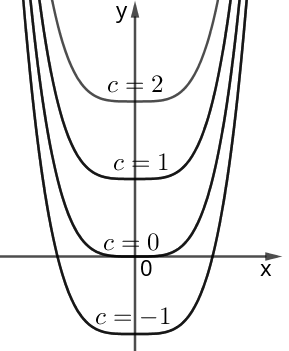
\includegraphics[width=0.3\linewidth]{5-Int_Indefinida/figs/FamiliaSolx^4.png}
%\label{SolRev}
}\qquad
\subfigure[b][]{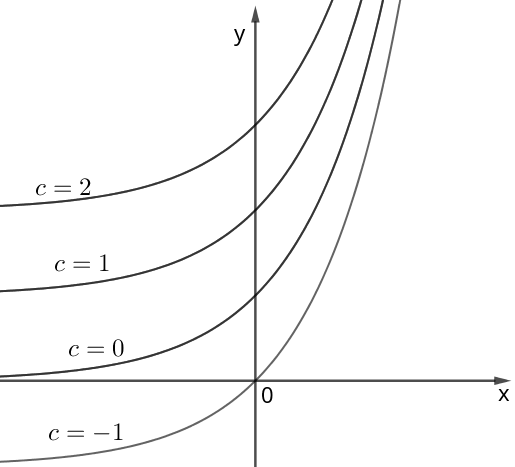
\includegraphics[width=0.45\linewidth]{5-Int_Indefinida/figs/Familia_antiDerivadae^x.png}
%\label{XR-XL}
}
%\caption{Representação de área limitada por curvas da forma $x=f(y)$ e $x=g(y)$}
%\label{fig:Area-entre-curvas-x=fy-gy}
\end{figure}
}

\begin{ex}
Determinemos as seguintes integrais indefinidas:
\begin{compactenum}[a)]
\item \item \(\intdef{}{}{x^2}\)

\begin{solution}
Desde que \(d\pc{\frac{x^3}{3}}=\frac{3x^2}{3}=x^2\), obtemos que

\[ \int x^2\, dx=\dfrac{x^3}{3}+c. \]
\end{solution}
\item \(\mathlarger{\int} \ln (x) dx\)

\begin{solution}
Desde que \(d(x\ln( x) -x)=\ln (x) dx\,\), obtemos que \(\mathlarger{\int} \ln (x) dx=x\ln (x)-x +c\).
\end{solution}

\end{compactenum}
\end{ex}

\begin{ex}
  Vejamos os seguintes casos:
  \begin{multicols}{2}
  \begin{enumerate}[a)]
  \item $\displaystyle \int \,dx = x + C$
  \item $\displaystyle \int 2x\,dx = x^2 + C$
  \item $\displaystyle \int \cos(x)\,dx = \sen(x) + C$
  \item $\displaystyle \int e^x\,dx = e^x + C$
  \end{enumerate}
  \end{multicols}
\end{ex}

\section{Regras básicas de integração}\label{sec:RegrasIntegracao}

Na Seção \ref{Cap:IntInd-sec:Antiderivada}, definimos a integral indefinida por
\begin{equation}
  \int f(x)\,dx = F(x) + C,
\end{equation}
onde $F$ é uma \emph{primitiva} de $f$, i.e. $F' = f$, e $C$ é uma \emph{constante indeterminada}. Na sequência, vamos discutir sobre as regras básicas para o cálculo de integrais.


\subsection{Multiplicação por constante e da soma/subtração}\label{subsec:DemSomaSubtracao}

Das regras de multiplicação por constante e da soma para derivadas, podemos concluir que
\begin{itemize}
\item $\displaystyle \boldsymbol{\int k\cdot f(x)\,dx = k\cdot \int f(x)\,dx},\quad k\neq 0$ constante.

  De fato, seja $F$ uma primitiva de $f$. Temos $(k\cdot F)' = k\cdot F' = k\cdot f$, i.e. $k\cdot F$ é primitiva de $k\cdot f$.
  
\item $\displaystyle \boldsymbol{\int \left[f(x)\pm g(x)\right]\,dx = \int f(x)\,dx \pm \int g(x)\,dx}$.

  De fato, sejam $F$ uma primitiva de $f$ e $G$ uma primitiva de $g$. Temos $(F + G)' = F' + G' = f + g$, i.e. $F + G$ é primitiva de $f+g$.
\end{itemize}

\begin{obs}
  Como $(x)' = 1$, temos que a \emph{integral de função constante} $f(x)\equiv k$ é
  \begin{equation*}
    \int k\,dx = k\int 1\cdot\,dx = k\cdot x + C
  \end{equation*}
\end{obs}

\begin{ex}
  Vejamos os seguintes casos:
  \begin{enumerate}[a)]
  \item
    \begin{align*}
      \int 2x\,dx &= 2\int x\,dx \\
                  &= 2 \left(\frac{x^2}{2} + C\right) \\
                  &= x^2 + C
    \end{align*}
  \item
    \begin{align*}
      \int (2x^2 - 3x + 1)\,dx &= \int 2x^2\,dx - \int 3x\,dx + \int \,dx \\
                               &= 2\int x^2\,dx - 3\int x\,dx + x + C \\
                               &= \frac{2}{3}x^3 - \frac{3}{2}x^2 + x + C
    \end{align*}
  \end{enumerate}
\end{ex}


\begin{ex}
Determinemos a seguinte integral indefinida \(\mathlarger{\int} (e^x-4x^3+\ln (x))dx\)

\begin{solution}
Pelas propriedades anteriores, temos que:

\[ \begin{array}{rcl} \mathlarger{\int} (e^x-4x^3+\ln (x))dx &=&\mathlarger{\int} e^xdx -\mathlarger{\int} 4x^3dx + \mathlarger{\int} \ln (x) dx\\ &=&(e^x+c_1)-(x^4+c_2)+(x\ln (x) - x+c_3)\\ &=& e^x-x^4+x\ln (x) - x+c \end{array} \]
onde \(c=c_1+c_2+c_3\).
\end{solution}
\end{ex}
\subsection{Integral de função potência}\hypertarget{IntFuncPot}{}\label{subsec:DemPotencia}

Com base na derivada de função potência, podemos afirmar que
\begin{equation}
  \boldsymbol{\int x^r\,dx = \frac{x^{r+1}}{r+1} + C,\quad r\neq -1}
\end{equation}
De fato, temos
\begin{equation*}
  \left(\frac{x^{r+1}}{r+1}\right)' = (r+1)\cdot \frac{x^r}{r+1} = x^r,
\end{equation*}
para $r\neq -1$.

\begin{ex}
  Vejamos os seguintes casos:
  \begin{enumerate}[a)]
  \item $\displaystyle \int x\,dx = \frac{x^2}{2} + C$.
  \item $\int x^2\,dx = \frac{x^3}{3} + C$
  \item $\displaystyle \int \frac{1}{x^2}\,dx = \int x^{-2}\,dx = -x^{-1} + C = -\frac{1}{x}+C$.
  \end{enumerate}
\end{ex}
\subsection{Integral de 1/x}\hypertarget{IntFunc1/x}{}\label{subsec:Dem-1/x}

A função logaritmo natural $y = \ln x$ é definida como a inversa da função exponencial natural $y = e^x$. Pode-se mostrar que
\begin{equation}
  \ln x = \int_1^x\frac{1}{t}\,dt,\quad x>0.
\end{equation}
Isto está de acordo com o fato de que da parte I do Teorema Fundamental do Cálculo, temos
\begin{equation}
  \frac{d}{dx}\ln x = \frac{1}{x}
\end{equation}
Agora, da Regra da cadeira temos
\begin{align*}
  \frac{d}{dx}\ln(-x) &= \frac{1}{-x}\frac{d(-x)}{dx} \\
                      &= \frac{1}{x}
\end{align*}
Com isso, podemos concluir que
\begin{equation}
  \boldsymbol{\int \frac{1}{x}\,dx = \ln|x| + C}
\end{equation}

\begin{ex}
  Vamos calcular
  \begin{equation*}
    \int_1^e \frac{1}{x}\,dx
  \end{equation*}
  Usando o Teorema Fundamental do Cálculo, temos
  \begin{align*}
    \int_1^e \frac{1}{x}\,dx &= \left. \ln x\right|_1^e \\
                             &= \ln(e) - \ln(1) \\
                             &= 1
  \end{align*}
\end{ex}
\begin{ex}
  Calcule
  \begin{equation*}
    \int \frac{1}{2x}\,dx
  \end{equation*}
  \begin{resol}
  Das regras básicas de integração, temos
  \begin{align*}
    \int \frac{1}{2x}\,dx &= \int \frac{1}{2}\cdot\frac{1}{x}\,dx \\
                          &= \frac{1}{2}\int\frac{1}{x}\,dx \\
                          &= \frac{1}{2}\ln(x) + C \\
                          &= \ln\sqrt{x} + C
  \end{align*}

No \geogebra, temos: \verb| integral(1/(2*x))|
\end{resol}
\end{ex}

\begin{ex}\label{ExDem:tInt-du/(u^2-a^2)}
Mostremos que

\[ \mathlarger{\int} \dfrac{du}{u^2-a^2} = \dfrac{1}{2a}\ln \left|\dfrac{u-a}{u+a} \right| +c, \quad \mbox{ para }a>0. \]

\begin{solution}
\[ \dfrac{d}{du}\left( \dfrac{1}{2a}\ln \left|\dfrac{u-a}{u+a} \right| \right)=\dfrac{1}{2a}\left[\dfrac{d}{du}( \ln |u-a|-\ln |u+a|) \right]= \dfrac{1}{2a}\left[\dfrac{1}{u-a}-\dfrac{1}{u+a} \right]=\dfrac{1}{u^2-a^2}. \]
Portanto, \(\mathlarger{\int} \dfrac{du}{u^2-a^2} = \dfrac{1}{2a}\ln \left|\dfrac{u-a}{u+a} \right| +c\).
\end{solution}
\end{ex}
\subsection{Integral da função exponencial natural}\hypertarget{IntExp}{}\label{subsec:Int_e^x}
Da derivada da função exponencial natural, temos
\begin{equation}
  \int e^x\,dx = e^x + C
\end{equation}

\begin{ex}
  \begin{align*}
    \int e^{2 + x}\,dx &= \int e^2e^x\,dx \\
                       &= e^2\int e^x\,dx \\
                       &= e^2e^x + C \\
                       &= e^{2+x} + C
  \end{align*}
\end{ex}

\subsection*{Tabela de integrais}
Segue abaixo as integrais que já anunciamos e praticamos até o momento. As integrais \eqref{eq:Intkf}  e \eqref{eq:IntSomaSub} foram demonstradas na subseção \ref{subsec:DemSomaSubtracao}. A Integral \ref{eq:IntPot}  foi demonstrada na subseção \ref{subsec:DemPotencia}, as integrais \eqref{eq:Int_1/x} foi demonstrada na subseção \ref{subsec:Dem-1/x} e \eqref{eq:Int-e^x} demostramos na subseção \ref{subsec:Int_e^x}. Demostramos a integral \eqref{eq:Int-a^x}  na subseção \ref{subc:Int-a^x}. Já a demostração da integral \eqref{eq:Int_u^2-a^2} foi feita no Exemplo \ref{ExDem:tInt-du/(u^2-a^2)}. 

\begin{align}
 \label{eq:Intkf}
 & \int k\cdot f(x)\,dx = k\cdot\int f(x)\,dx\\\label{eq:IntSomaSub}
  & \int \left[f(x)\pm g(x)\right]\,dx = \int f(x)\,dx \pm \int g(x)\,dx\\\label{eq:IntPot}
  & \int x^r\,dx = \frac{x^{r+1}}{r+1} + C,\quad r\neq -1\\\label{eq:Int_1/x}
  & \int \frac{1}{x}\,dx = \ln x + C \\\label{eq:Int-e^x}
  & \int e^x\,dx = e^x + C\\\label{eq:Int-a^x}
  & \int a^x\,dx = \frac{a^x}{\ln a} + C\\\label{eq:Int_u^2-a^2}
  & \int \frac{du}{u^2-a^2} = \frac{1}{2a}\ln \left|\dfrac{u-a}{u+a}\right|
   \end{align}

\subsection{Exercícios Resolvidos}
\begin{exeresol}
  Determinemos as seguintes integrais indefinidas:
  \begin{compactenum}[a)]
  \item \(\mathlarger{\int} x(a-bx^2)dx\), para \(a,\,b\in \mathbb{R}\).
  
  \begin{solution}
  \[ \mathlarger{\int} x(a-bx^2)dx= \mathlarger{\int} (ax-bx^3)dx= a\mathlarger{\int} x dx -b \mathlarger{\int}x^3 dx= \dfrac{ax^2}{2} - \dfrac{bx^4}{4}+c. \]
  \end{solution}
  \item \(\mathlarger{\int} \dfrac{(x^m -x^n)^2}{\sqrt{x}}dx\), onde \(m,\,n\neq \dfrac{3}{4}\) e \(m+n\neq \dfrac{3}{2}\).
  
  \begin{solution}
  Antes de determinar essa integral, precisamos reescrever \(f\):

\[ \dfrac{(x^m -x^n)^2}{\sqrt{x}}=\dfrac{x^{2m}-2x^{m+n} +x^{2n}}{\sqrt{x}} = x^{2m-\frac{1}{2}}-2x^{m+n-\frac{1}{2}} + x^{2n-\frac{1}{2}}= x^{\frac{4m-1}{2}}-2x^{\frac{2m+2n-1}{2}}+x^{\frac{4n-1}{2}}. \]
Logo,

\[ \begin{array}{rcl} \mathlarger{\int} \dfrac{(x^m -x^n)^2}{\sqrt{x}}dx &=& \mathlarger{\int} \left(x^{\frac{4m-1}{2}}-2x^{\frac{2m+2n-1}{2}}+x^{\frac{4n-1}{2}}\right)dx\\ &=& \mathlarger{\int} x^{\frac{4m-1}{2}} dx -2 \mathlarger{\int} x^{\frac{2m+2n-1}{2}}dx + \mathlarger{\int}x^{\frac{4n-1}{2}}dx\\ \\ &=& \dfrac{x^{\frac{4m+1}{2}}}{\frac{4m+1}{2}} - 2\dfrac{x^{\frac{2m+2n+1}{2}}}{\frac{2m+2n+1}{2}} + \dfrac{x^{\frac{4n+1}{2}}}{\frac{4n+1}{2}} + c\\ \\ &=& \dfrac{2\sqrt{x^{4m+1}}}{4m+1} - \dfrac{4\sqrt{x^{2m+2n+1}}}{2m+2n+1} + \dfrac{2\sqrt{x^{4n+1}}}{4n+1} + c. \end{array} \]
  \end{solution}
  \end{compactenum}
  
\end{exeresol}
\subsection{Exercícios}

\begin{exer}
  Calcule
  \begin{multicols}{4}
  \begin{enumerate}[a)]
  \item $\displaystyle \int \,dx$
  \item $\displaystyle \int x^{-2}\,dx$
  \item $\displaystyle \int \sqrt{x}\,dx$
  \item $\displaystyle \int \frac{1}{\sqrt{x}}\,dx$
  \end{enumerate}\end{multicols}
\end{exer}
\begin{resp}
  a)~$\displaystyle x + C$; b)~$\displaystyle -\frac{1}{x} + C$; c)~$\displaystyle \frac{2}{3}x^{3/2} + C$; d)~$\displaystyle 2x^{1/2} + C$
\end{resp}

\begin{exer}
  Calcule
   \begin{multicols}{3}
  \begin{enumerate}[a)]
  \item $\int x^3\,dx$
  \item $\displaystyle \int 1 + x^{-2}\,dx$
  \item $\displaystyle \int x - \frac{1}{x}\,dx$
    \end{enumerate}\end{multicols}
\end{exer}
\begin{resp}
 a) $\frac{x^4}{4}$; b)~$\displaystyle x-\frac{1}{x}+C$; c)~$\displaystyle \frac{x^2}{2} - \ln|x| + C$
\end{resp}

\section{Técnicas de Integração}
\subsection{Integração por substituição}\hypertarget{IntSubst}{}\label{sec:MetSubst}
Em alguns casos, é necessário fazer uma mudança de variável no integrando com o intuito de torná-lo mais simples de ser resolvido. A necessidade ou não de fazer tal mudança é consequência da complexidade da integral a ser calculada. Com a prática você perceberá se é necessário ou não aplicar esta técnica nas integrais a serem resolvidas. Técnica esta chamada de Método da Substituição, o qual mostraremos abaixo.

Seja $u = u(x)$. A regra de integração por substituição é
\begin{equation}
  \boldsymbol{\int f(u(x))u'(x)\,dx = \int f(u)\,du}
\end{equation}
De fato, se
\begin{equation}
  \int f(u)\,du = F(u) + C,
\end{equation}
então, da regra da cadeira (Seção \ref{Chap:RegraCadeia}), temos
\begin{align*}
  \frac{d}{dx}F(u(x)) &= F'(u(x))u'(x) \\
                      &= f(u(x))u'(x),
\end{align*}
i.e. $F(u(x))$ é primitiva de $f(u(x))u'(x)$.

\begin{ex}
  Vejamos os seguintes casos:
  \begin{enumerate}[a)]
  \item $\displaystyle\int 2(2x+1)^2\,dx$.
    
    Tomamos $f(u) = u^2$ com $u(x) = 2x+1$, donde $u'(x) = 2$. Logo
    \begin{align*}
      \int 2(2x+1)^2\,dx &= \int f(u(x))u'(x)\,dx \\
                         &= \int f(u)\,du \\
                         &= \int u^2\,du \\
                         &= \frac{u^3}{3} + C \\
                         &= \frac{(2x+1)^3}{3} + C
    \end{align*}
     \item $ \int (2x+1)^2\,dx$
  
    Substituindo
  \begin{equation*}
    u = 2x+1
  \end{equation*}
  temos
  \begin{equation*}
    \frac{du}{dx} = 2 \Rightarrow dx = \frac{du}{2}
  \end{equation*}
  Portanto,
  \begin{align*}
    \int (2x+1)^2\,dx &= \int u^2\,\frac{du}{2}\\
                     &= \frac{1}{2}\int u^2\,du\\
                     &= \frac{1}{2}\frac{u^{2+1}}{2+1} + C\\
                     &= \frac{u^3}{6} + C\\
                     &= \frac{1}{6}(2x+1)^3 + C
  \end{align*}
  \item $ \int \frac{7}{(x-1)^2}\,dx$

  Usamos a regra de integração por substituição
  \begin{equation*}
    \int f(u(x))u'(x)\,dx = \int f(u)\,du.
  \end{equation*}
  Escolhemos
  \begin{equation*}
    u = x-1,
  \end{equation*}
  e calculamos
  \begin{equation*}
    \frac{du}{dx} = 1 \Rightarrow du = dx
  \end{equation*}
  Então, da fórmula, obtemos
  \begin{align*}
    \int \frac{7}{(x-1)^2}\,dx &= \int \frac{7}{u^2}\,du\\
                               &= 7\int u^{-2}\,du\\
                               &= 7\frac{u^{-2+1}}{-2+1}\\
                               &= -\frac{7}{u}\\
                               &= \frac{7}{1-x}
  \end{align*}

\item $ \int \frac{e^x}{e^x - 1}\,dx$

  Fazendo a substituição
  \begin{equation*}
    u = e^x-1 \Rightarrow du = e^x\,dx,
  \end{equation*}
  temos
  \begin{align*}
    \int \frac{e^x}{e^x - 1}\,dx &= \int \frac{1}{u}\,du \\
                                 &= \ln|u| + C \\
                                 &= \ln|e^x-1|+C
  \end{align*}

  No \geogebra~podemos resolver com o comando: \verb| integral(exp(x)/(exp(x)-1))|

\item $\displaystyle\int \pi\sen(\pi x)\,dx$.
    
    Tomando $f(u)=\sen(u)$, $u=\pi x$, temos $u'(x)=\pi$. Logo
    \begin{align*}
      \int \pi\sen(\pi x)\,dx &= \int f(u(x))u'(x)\,dx \\
                              &= \int f(u)\,du \\
                              &= \int \sen(u)\,du \\
                              &= -\cos(u) + C \\
                              &= -\cos(\pi x) + C
    \end{align*}
   \end{enumerate}
\end{ex}
\subsection*{Integral de função exponencial}\label{subc:Int-a^x}

Na Subseção \ref{subsec:Int_e^x}, vimos que
\begin{equation*}
  \int e^x\,dx = e^x + C
\end{equation*}
Agora, com a regra da substituição, temos
\begin{align*}
  \int a^x\,dx &= \int e^{\ln a^x}\,dx \\
               &= \int e^{x\ln a}\,dx,
\end{align*}
com $a>0$ e $a\neq 1$. Tomando
\begin{equation*}
  u = x\ln a \Rightarrow du = \ln(a)dx
\end{equation*}
Segue que
\begin{align*}
  \int a^x\,dx &= \int e^u\frac{du}{\ln a} \\
               &= \frac{1}{\ln a}\int e^u\,du \\
               &= \frac{e^u}{\ln a} + C \\
               &= \frac{e^{x\ln a}}{\ln a} + C \\
               &= \frac{e^{\ln a^x}}{\ln a} + C \\
               &= \frac{a^x}{\ln a} + C
\end{align*}
Ou seja, concluímos que
\begin{equation}
  \boldsymbol{\int a^x\,dx = \frac{a^x}{\ln a} + C}
\end{equation}

\begin{ex}
  Vamos calcular
  \begin{equation*}
    \int x\cdot 2^{x^2}\,dx
  \end{equation*}
  Por substituição, tomamos
  \begin{equation*}
    u = x^2 \Rightarrow du = 2xdx,
  \end{equation*}
  segue
  \begin{align*}
    \int x\cdot 2^{x^2}\,dx &= \int \cdot 2^{u}\frac{du}{2} \\
                            &= \frac{1}{2}\int \cdot 2^{u}\,du \\
                            &= \frac{1}{2}\frac{2^u}{\ln 2} + C \\
                            &= \frac{1}{2}\frac{2^{x^2}}{\ln 2} + C
  \end{align*}
\end{ex}
\subsubsection{Exercícios Resolvidos}
\begin{exeresol}
  Determinemos as seguintes integrais indefinidas:
  \begin{compactenum}[a)]
  \item  \(\mathlarger{\int} (x^3+1)^4 3x^2dx\)
  
  \begin{solution}
  Fazendo \(u=x^3+1\), temos que \(du=3x^2 dx\). Logo,

\[ \mathlarger{\int} (x^3+1)^4 3x^2dx= \mathlarger{\int} u^4du=\dfrac{t^5}{5}+c=\dfrac{(x^3+1)^5}{5}+c. \]
  \end{solution}
  \item \(\mathlarger{\int} \dfrac{x^4}{\sqrt[7]{x^5+1}}dx\)
  
  \begin{solution}
  Fazendo \(u=x^5+1\), obtemos que \(du=5x^4dx\), então,

\[ \mathlarger{\int} \dfrac{x^4}{\sqrt[7]{x^5+1}}dx=\dfrac{1}{5}\mathlarger{\int} \dfrac{5x^4dx}{\sqrt[7]{x^5+1}}= \dfrac{1}{5}\mathlarger{\int} u^{-1/7}du=\dfrac{1}{5}\cdot\dfrac{7}{6}u^{6/7}+c=\dfrac{7}{30}\sqrt[7]{(x^5+1)^6}+c. \]
  \end{solution}
  \item \(\mathlarger{\int} \dfrac{5e^x}{\sqrt{1-e^{2x}}}dx\)\\
  
  \begin{solution}
  Fazendo \(u=e^x\), obtemos que \(du=e^xdx\), então,

\[ \mathlarger{\int} \dfrac{5e^x}{\sqrt{1-e^{2x}}}dx=5\mathlarger{\int} \dfrac{du}{\sqrt{1-u^{2}}}=5\,{\rm arcsen\,}(u)+c=5\,{\rm arcsen\,}(e^x)+c. \]
  \end{solution}
  \item \(\mathlarger{\int} \dfrac{{\rm senh}(x)\,\cosh(x) }{(1+{\rm senh}^2 (x))^5}dx\)
  
  \begin{solution}
  Fazendo \(u=1+{\rm senh}^2 (x)\), obtemos que \(du=2\,{\rm senh}(x) \cosh (x) dx\), então,
\[ \mathlarger{\int} \dfrac{{\rm senh}(x)\,\cosh( x) }{(1+{\rm senh}^2 (x))^5}= \mathlarger{\int} \dfrac{\frac{1}{2}du}{u^5}=\dfrac{1}{2}\mathlarger{\int} u^{-5}du = \dfrac{1}{2}\dfrac{u^{-4}}{(-4)} +c =\dfrac{-1}{8(1+{\rm senh}^2 (x))^4}+c. \]
  \end{solution}
  \item \( \mathlarger{\int} \dfrac{x+2}{(x-2)^4}dx\)\\
  
  \begin{solution}
  Fazendo \(u=x-2\), obtemos que \(du=dx\). Logo,
\[ \mathlarger{\int} \dfrac{u+4}{u^4}du= \mathlarger{\int} (u^{-3}+4u^{-4})du=-\dfrac{1}{2}u^{-2}-\dfrac{4}{3}u^{-3}+c = -\dfrac{3x+2}{6(x-2)^3}+c. \]
  \end{solution}
  \item \( \mathlarger{\int} x\sqrt{x+4}\,dx\)
  
  \begin{solution}
  Fazendo \(u=\sqrt{x+4}\), obtemos que \(u^2=x+4\) e \(dx=2u du\). Logo,

\[ \begin{array}{rcl} \mathlarger{\int} x\sqrt{x+4}\,dx &=& \mathlarger{\int}(u^2-4)\,u\,2u\, du = \mathlarger{\int}(2u^4-8u^2)du\\ &=&\dfrac{2}{5}u^5-\dfrac{8}{3}u^3 +c =\dfrac{u^3}{15}(6u^2-40)+c =\dfrac{(x+4)^{3/2}}{15}(6x-16)+c. \end{array} \]
  \end{solution}
  \end{compactenum}
 \end{exeresol}
\nota{As vezes é necessário manipular a forma da função a ser integrada e obter uma expressão equivalente, novamente, com o intuito de facilitar a determinação da integral. É o que veremos nos próximos exemplos.}
\begin{exeresol}
  \begin{compactenum}[a)]
  \item \(\mathlarger{\int}\dfrac{x}{e^{3x}(1-x)^4} dx\)\\
 
  \begin{solution}
   Notamos que no integrando, o denominador pode ser reescrito como uma potência. De fato, multiplicando tanto o numerador como o denominador por \(e^x\), temos que:

\[ \dfrac{x}{e^{3x}(1-x)^4} =\dfrac{xe^x}{(e^{3x}(1-x)^4)e^x} =\dfrac{xe^x\,}{e^{4x}(1-x)^4}=\dfrac{xe^x}{(e^x-xe^x)^4}, \]
assim, fazendo \(u=e^x-xe^x\), obtemos \(du=-xe^x dx\) ou, equivalentemente, \(-du=xe^x dx\), o que resulta em:

\[ \mathlarger{\int}\dfrac{x}{e^{3x}(1-x)^4} dx=\mathlarger{\int}\dfrac{xe^x \,dx}{\left(e^{x}-xe^x \right)^4} dx =-\mathlarger{\int}\dfrac{du}{u^4}=\dfrac{1}{3u^3}+c = \dfrac{1}{3e^{3x}(1-x)^3} +c. \]
  \end{solution}
  \item \( \mathlarger{\int} \dfrac{(x^2-1)dx}{(x^2+1)\sqrt{x^4+1}}\)\\
  
  \begin{solution}
  Novamente, dividindo o numerador e o denominador do integrando por \(x^2\), obteremos:

\[ \dfrac{(x^2-1)}{(x^2+1)\sqrt{x^4+1}}=\dfrac{\dfrac{x^2-1}{x^2}}{\left(\dfrac{x^2+1}{x}\right)\dfrac{\sqrt{x^4+1}}{x}} = \dfrac{\left(1 -\dfrac{1}{x^2}\right)}{\left( x+\dfrac{1}{x}\right)\sqrt{x^2+\dfrac{1}{x^2}}}. \]
Fazendo \(u=x+\dfrac{1}{x}\), temos que \(du=\left(1 -\dfrac{1}{x^2}\right)dx\) e \(\quad u^2-2=x^2+\dfrac{1}{x^2}\). Logo,

\[ \mathlarger{\int} \dfrac{(x^2-1)dx}{(x^2+1)\sqrt{x^4+1}} = \mathlarger{\int} \dfrac{\left(1 -\dfrac{1}{x^2}\right)\,dx}{\left( x+\dfrac{1}{x}\right)\sqrt{x^2+\dfrac{1}{x^2}}} =\mathlarger{\int}\dfrac{du}{u\sqrt{u^2-2}}=\dfrac{1}{\sqrt{2}}{\rm arcsen}\dfrac{|u|}{\sqrt{2}}+c. \]
Portanto,

\[ \mathlarger{\int} \dfrac{(x^2-1)dx}{(x^2+1)\sqrt{x^4+1}}=\dfrac{1}{\sqrt{2}}{\rm arcsen}\left(\dfrac{x^2+1}{\sqrt{2}|x|} \right)+c. \]
  \end{solution}
  \item \(\mathlarger{\int} \dfrac{x dx}{\sqrt{1+x^2+\sqrt{(1+x^2)^3}}}\)
  
  \begin{solution}
  Manipulando o integrando, temos que ele pode ser reescrito como \(\dfrac{x}{\sqrt{1+x^2}\sqrt{1 +\sqrt{1+x^2}}}\). Logo, fazendo \(u=1 +\sqrt{1+x^2}\), obteremos \(du=\dfrac{x dx}{\sqrt{1+x^2}}\). Assim,

\[ \mathlarger{\int} \dfrac{x}{\sqrt{1+x^2}\sqrt{1 +\sqrt{1+x^2}}}dx= \mathlarger{\int} \dfrac{du}{\sqrt{u}}= \mathlarger{\int} u^{-1/2}du = 2\sqrt{u}+c. \]
Portanto,

\[ \mathlarger{\int} \dfrac{x dx}{\sqrt{1+x^2+\sqrt{(1+x^2)^3}}}= 2\sqrt{1 +\sqrt{1+x^2}} +c. \]
  \end{solution}
  \end{compactenum}
\end{exeresol}
\subsection{Integral de funções trigonométricas}\hypertarget{IntTrig}{}
Nesta subseção, usaremos alguns artifícios para resolver algumas integrais que envolvem funções trigonométricas e, para isto, será necessário lembrar das seguintes identidades:
\begin{multicols}{2}
1. \(\quad \sen^2(u)+ \cos^2(u)=1 \);

2. \(\quad{\rm sec}^2(u)- {\rm tg} ^2(u)=1 \);

3. \(\quad{\rm cossec}^2(u) - {\rm cotg}^2(u)=1 \);

4. \(\quad\sen^2(u) = \dfrac{1- \cos(2u)}{2}\);

5. \(\quad\cos^2(u) = \dfrac{1+ \cos(2u)}{2}\);
\end{multicols}
%\section[\texorpdfstring{This $a^2 + b^3$ equation looks fine}{Some variant with no TeX}]{\boldmat{ This $a^2 + b^3$ equation looks tem }}

\subsubsection[\formula{Integrais de  $\sin x, \cos x$ e  $\tg x$}]{\boldmat{Integrais de  $\sin x, \cos x$ e  $\tg x$}}
Com base na derivada de funções trigonométricas, temos

  \begin{equation}
    \boldsymbol{\int \sen(x)\,dx = -\cos(x) + C}
  \end{equation}
De fato, $\mathit{\pc{-\cos x+C}'=-(\cos x)'+C'=-(-\sin x)=\sin x}$
  \begin{equation}
    \boldsymbol{\int \cos(x)\,dx = \sen(x) + C}
  \end{equation}
De fato, $\mathit{\pc{\sin x+C}'=(\sin x)'+C'=\cos x}$

Para determinar $ \int \tg(x)\,dx$, primeiro consideramos que $\tg(x)=\frac{\sin x}{\cos x}$ e então utilizamos o método da substituição, como segue:

\begin{align*}
  \int \tg(x)\,dx &= \int \frac{\sen(x)}{\cos(x)}\,dx
\end{align*}
Escolhendo
\begin{equation*}
  u = \cos(x) \Rightarrow du = -\sen(x)\,dx
\end{equation*}
Fazendo a substituição e calculando, temos
\begin{align*}
  \int \tg(x)\,dx &= -\int \frac{1}{u}\,du \\
                  &= -\ln|u| + C \\
                  &= -\ln|\cos(x)| + C \\
                  &= \ln\left|\frac{1}{\cos(x)}\right| + C\\
                  &= \ln|\sec(x)| + C
\end{align*}
Ou seja, concluímos que
\begin{equation}
  \boldsymbol{\int\tg(x)\,dx = \ln|\sec(x)| + C}
\end{equation}

\begin{ex}
  Vamos calcular
  \begin{equation*}
    \int_0^{\pi} \cos(x) - \sen(x)\,dx
  \end{equation*}
  \begin{sol}
  Temos
  \begin{align*}
    \int \cos(x)-\sen(x)\,dx &= \int\cos(x)\,dx - \int\sen(x)\,dx\\
                             &= \sen(x) + \cos(x) + C
  \end{align*}
  Agora, do Teorema Fundamental do Cálculo, obtemos
  \begin{align*}
    \int_0^{\pi} \cos(x)-\sen(x)\,dx &= \left.\sen(x) + \cos(x)\right|_0^\pi \\
                             &= \sen(\pi)+\cos(\pi) - \left[\sen(0)+\cos(0)\right]\\
                             &= -1 - 1 = -2.
  \end{align*}
  \end{sol}
\end{ex}

\begin{ex}
  Vamos calcular
  \begin{equation*}
    \int \sen\!\!^2(x)\,dx
  \end{equation*}
  \begin{sol}
  Usando a identidade trigonométrica \ref{eq:SenDuplo}, temos
  \begin{align}
    \int \sen\!\!^2(x)\,dx &= \int \frac{1-\cos(2x)}{2}\,dx\nonumber \\
                       &= \frac{1}{2}\int\,dx - \frac{1}{2}\int\cos(2x)\,dx\label{int_subs_aux1}
  \end{align}
  Agora, tomando $u = 2x$, temos $du = 2\,dx$, donde
  \begin{align*}
    \int \cos(2x)\,dx &= \int\cos(u)\frac{du}{2}\nonumber \\
                      &= \frac{1}{2}\sen(u) + C\nonumber \\
                      &= \frac{1}{2}\sen(2x) + C
  \end{align*}
  Retornando a \ref{int_subs_aux1}, obtemos
  \begin{align}
    \boldsymbol{\int \sen\!\!^2(x)\,dx = \frac{x}{2} - \frac{\sen(2x)}{4} + C}
  \end{align}
  \end{sol}
\end{ex}

\begin{ex}
  Vamos calcular
  \begin{equation*}
    \int x\tg(x^2)\,dx
  \end{equation*}
  \begin{sol}
  Usando a regra de substituição, escolhemos
  \begin{equation*}
    u = x^2 \Rightarrow du = 2x\,du.
  \end{equation*}
  Fazendo a substituição e calculando, obtemos
  \begin{align*}
    \int x\tg(x^2)\,dx &= \int \tg(u)\,\frac{du}{2} \\
                       &= \frac{1}{2}\int \tg(u)\,du \\
                       &= \frac{1}{2}\ln|\sec(u)| + C \\
                       &= \frac{1}{2}\ln|\sec(x^2)| + C
  \end{align*}
  \end{sol}
\end{ex}
\subsubsection[\formula{Integral das funções $\sec x$, $\cossec x$ e $\cotg x$}]{\boldmat{Integral das funções $\sec x$, $\cossec x$ e $\cotg x$}}
Agora, vamos calcular
\begin{equation*}
  \int \sec(x)\,dx
\end{equation*}

Observamos que
\begin{align*}
  \int\sec(x)\,dx &= \int \sec(x)\cdot\frac{\sec(x)+\tg(x)}{\sec(x)+\tg(x)}\,dx \\
                  &= \int \frac{\sec^2(x)+\sec(x)\tg(x)}{\sec(x)+\tg(x)}\,dx
\end{align*}
Então, fazendo a substituição
\begin{equation*}
  u = \sec(x) + \tg(x) \Rightarrow du = \sec(x)\tg(x) + \sec^2(x),
\end{equation*}
temos
\begin{align*}
  \int\sec(x)\,dx &= \int\frac{\sec^2(x)+\sec(x)\tg(x)}{\sec(x)+\tg(x)}\,dx \\
                  &= \int\frac{1}{u}\,du \\
                  &= \ln|u| + C \\
                  &= \ln|\sec(x)+\tg(x)| + C
\end{align*}
Ou seja, obtemos
\begin{equation}
  \boldsymbol{\int\sec(x)\,dx = \ln|\sec(x)+\tg(x)|+C}
\end{equation}
\begin{obs}
Com raciocínio análogo ao utilizado na integração da função secante, obtemos\footnote{Veja o Exercício \ref{exer:int_subs_cossec}.}
\begin{equation}
  \boldsymbol{\int \cossec(x)\,dx = -\ln|\cossec(x)+\cotg(x)| + C}
\end{equation}
\end{obs}

\begin{obs}
Com raciocínio análogo ao utilizado na integração da função tangente, obtemos\footnote{Veja o Exercício \ref{exer:int_subs_cotg}.}
\begin{equation}
  \boldsymbol{\int \cotg(x)\,dx = \ln|\sen(x)| + C}
\end{equation}
\end{obs}

\begin{ex}
  Vamos calcular
  \begin{equation*}
    \int\sec\left(\frac{u}{2}\right)\,du.
  \end{equation*}
  \begin{sol}
  Fazendo a substituição
  \begin{equation*}
    v = \frac{u}{2} \Rightarrow dv = \frac{du}{2},
  \end{equation*}
  segue
  \begin{align*}
    \int\sec\left(\frac{u}{2}\right)\,du &= \int\sec(v)\cdot 2\,dv \\
                                         &= 2\int \sec(v)\,dv \\
                                         &= 2\ln|\sec(v)+\tg(v)| + C \\
                                         &= 2\ln\left|\sec\left(\frac{u}{2}\right)+\tg\left(\frac{u}{2}\right)\right| + C
  \end{align*}
  \end{sol}
\end{ex}

\subsubsection{Integrais tipo \texorpdfstring{$\int \sin\!\!^m \cos^n\, dx$}{}}
Muitas funções trigonométricas podem ser integradas combinando substituição e integração
por partes com as identidades trigonométricas apropriadas. Primeiro, considere
$$\int \sin\!\!^m \cos^n\, dx$$
onde $m, n$ são números inteiros. O caso mais fácil é quando pelo menos um de $m, n$ é ímpar. 
\paragraph*{Caso I: Um dos expoentes \(m\) ou \(n\) é um inteiro positivo ímpar}
\begin{compactenum}[i.]
\item Se \(m\) é um número ímpar e \(n\) é qualquer número, então expressamos a integral da seguinte forma:
\[ \begin{array}{lcl} \mathlarger{\int}\sen^m(x) \cos^n(x)\,dx &=& \mathlarger{\int}\sen^{m-1}( x) \cos^n (x)\,\sen (x)\,dx\end{array} \]
\item Se \(n\) é um número ímpar e \(m\) é qualquer número, então expressamos a integral da seguinte forma:

\[ \begin{array}{lcl} \mathlarger{\int}\sen^m (x) \cos^n(x)\,dx &=& \mathlarger{\int}\sen^{m}( x) \cos^{n-1} (x)\,\cos (x)\,dx\\ \end{array} \]
\end{compactenum}
Vamos ver alguns exemplos.
\begin{ex}[\pmb{Potência de $\sin x$ é impar}]~
 \\  Calcule \\
 \begin{compactenum}
 \item $\int \sin\!\!^3 x\, dx$.
 
    \begin{sol}
      Como $\sin\!\!^3 x$ é uma potência ímpar, a identidade $\sin\!\!^2 x = 1 - \cos\!\!^2 x$ nos permite  dividir  $\sin\!\!^3 x$ em fatores:
      $$\sin\!\!^3 x\, dx=\sin\!\!^2 x(\sin x\,dx)=(1-\cos^2 x)\sin x dx$$
      e utilizar a substituição $u=\cos x$, $du=-\sin x dx$:
      \begin{align*}
          \int \sin\!\!^3 x\, dx&=\int (1-\cos^2 x)\sin x dx=-\int (1-u^2)\, du\\
          &=\frac{u^3}{3}-u+C=\frac{\cos^3 x}{3}-\cos x+C
      \end{align*}
    \end{sol}
 \item \(\mathlarger{\int}\sen^3(x) \cos^4 (x)\,dx\)\\
   
   \begin{solution}
   \[ \begin{array}{rcl} \mathlarger{\int}\sen^3(x) \cos^4 (x)\,dx&=&\mathlarger{\int}\sen^3( x) \cos^4(x)\,dx = \mathlarger{\int}\left(\sen^2 (x) \cos^4( x)\,\right)\sen(x)\,dx\\ & =&\mathlarger{\int}\left((1-\cos^2 (x))\cos^4 (x)\,\right)\sen(x)\,dx. \end{array} \]
Na última integral, fazemos \(u=\cos(x) \), então \(du= - \sen(x)\,dx\). Portanto,

\[ \begin{array}{rcl} \mathlarger{\int}\sen^3(x) \cos^4(x)\,dx &=&\mathlarger{\int}(1-u^2)u^4(-du)= -\mathlarger{\int}(u^4-u^6)du=-\dfrac{u^5}{5}+\dfrac{u^7}{7}+c\\ &=& \dfrac{\cos^5(x)}{35}(5\cos^2(x)-7)+c. \end{array} \]
   \end{solution}
 \end{compactenum}
 
 
\end{ex}
\begin{ex}[\pmb{Potência de $\cos x$ é impar}]~
 Calcule $\int \sin\!\!^4 x\cos^5 x\, dx$.

 \begin{sol}
     Aproveitamos o fato de que $\cos^5 x$ é uma potência ímpar para escrever
     $$ \sin\!\!^4 x\cos^5 x\, dx= \sin\!\!^4 x\cos^4 x(\cos x\, dx)= \sin\!\!^4 x (1-\sin^2 x)^2(\cos x\, dx)$$. 
     Isso nos permite utilizar a substituição $u=\sin x$, $du=\cos x\, dx$:
     \begin{align*}
         \int \sin\!\!^4 x\cos^5 x\, dx&=\int (\sin\!\!^4 x) (1-\sin^2 x)^2 \cos x\, dx\\
         &=\int u^4(1-u^2)^2\, du=\int (u^4-2u^6+u^8)\, du\\
         &=\frac{u^5}{5}-\frac{2u^7}{7}+\frac{u^9}{9}+C=\frac{\sin\!\!^5 x}{5}-\frac{2\sin\!\!^7 x}{7}+\frac{\sin\!\!^9 x}{9}+C
     \end{align*}
   \end{sol}
 
    
  
\end{ex}

As fórmulas de redução a seguir podem ser usadas para integrar $\sin x$ e $\cos x$ para qualquer expoente $n$, par ou ímpar (suas provas são deixadas como exercícios; veja Exercício 64 do livro de \citeonline{SmithCalculus}).
\begin{framed}
\textbf{Fórmulas de redução para seno e cosseno}
\begin{align}
    \sin\!\!^n x\, dx=-\frac{1}{n}\sin\!\!^{n-1}\, x \cos x+\frac{n-1}{n}\int \sin\!\!^{n-2} x\, dx\label{eq:FormRedSin^n}\\
    \cos^n x\, dx=\frac{1}{n}\cos^{n-1} x\, \sin\!\! x+\frac{n-1}{n}\int \cos^{n-2} x\, dx\label{eq:FormRedCos^n}
\end{align}
\end{framed}
\begin{ex}
  Calcule $\int \sin\!\!^4\, dx$
  \begin{solution}
    Aplicando a equação \eqref{eq:FormRedSin^n} com $n=4$,
    \begin{equation}
        \int \sin\!\!^4\, dx=-\frac{1}{4}\sin\!\!^3\, x\cos x+\frac{3}{4}\int \sin\!\!^2 x\, dx\label{eq:intsin^4ex}
    \end{equation}
       Então aplicando a Eq. \eqref{eq:FormRedSin^n} novamente na integral da direita:
    \begin{equation}
        \int \sin\!\!^2 x\, dx=-\frac{1}{2}\sin\!\!\, x\cos x+\frac{1}{2}\int  dx=-\frac{1}{2}\sin\!\!\, x\cos x+\frac{1}{2}x+C\label{eq:intsin^2ex}
    \end{equation}
    Usando as Equações \eqref{eq:intsin^4ex} e \eqref{eq:intsin^2ex}, obtemos
    \begin{equation*}
         \int \sin\!\!^4\, dx=-\frac{1}{4}\sin\!\!^3\, x\cos x-\frac{3}{8}\sin\!\!\, x\cos x+\frac{3}{8}x+C
    \end{equation*}
  \end{solution}
\end{ex}

\paragraph*{Caso II: Os expoentes \(m\) ou \(n\) são inteiros pares}
\begin{compactenum}[i.]
\item Se $m\leq n$, use a identidade $\sin\!\!^2 x = 1 - \cos^2 x$ para escrever
\begin{align}
    \int \sin\!\!^m x \cos^n x\, dx&=\int (\sin\!\!^2)^{m/2} x \cos^n x\, dx\nonumber\\
    &=\int (1 - \cos^2 x)^{m/2}\cos^n x\, dx
\end{align}
Expanda a integral à direita para obter uma soma das integrais de potências de $\cos x$ e use a fórmula de redução \eqref{eq:FormRedCos^n}.

\item Se $m\geq n$, use a identidade $\cos^2 x = 1 - \sin\!\!^2 x$ para escrever
\begin{align}
    \int \sin\!\!^m x \cos^n x\, dx&=\int \sin\!\!)^m x (\cos^2)^{n/2} x\, dx\nonumber\\
    &=\int \sin\!\!^m (1 - \sin\!\!^2 x)^{n/2}\, dx
\end{align}
Expanda a integral à direita para obter uma soma das integrais de potências de $\sin x$ e use a fórmula de redução (\ref{eq:FormRedSin^n}).
\end{compactenum}
\begin{ex}[\pmb{Potências de $\sin x$ e $\cos x$ são pares}]~
\\ Calcule $\int\sin\!\!^2 x\cos^4 x\, dx$
\begin{sol}
Temos que \(m=2\) e \(n=4\). Como \(m< n\), substituímos \(\sin\!\!^2 x\) por \(1-\cos^2 x\):
\begin{equation}
    \int\sin\!\!^2 x\cos^4 x\, dx=\int (1-\cos^2 x)\cos^4 x\, dx=\int \cos^4\, dx-\int \cos^6 x\, dx\label{eq:sen^2cos^4}
\end{equation}
A fórmula de redução para $n=6$ fornece:
 \begin{equation*}
   \intg{\cos^6 x}=\frac{1}{6}\cos^5 x\sin x+\frac{5}{6}\intg{\cos^4 x}
\end{equation*}
Usando o resultado do lado direito da Eq. (\ref{eq:sen^2cos^4}), nós obtemos
\begin{align*}
     \int\sin\!\!^2 x\cos^4 x\, dx & =\int \cos^4\, dx-\pc{\frac{1}{6}\cos^5 x\sin x+\frac{5}{6}\intg{\cos^4 x}}\\
     &=-\frac{1}{6}\cos^5x \sin x+\frac{1}{6}\intg{\cos^4 x}
\end{align*}
Agora nós avaliamos $\intg{\cos^4}$ utilizando a fórmula de redução \ref{eq:FormRedCos^n}:
\begin{align*}
    \intg{\cos^4 x}&=\frac{1}{4}\cos^3 x\sin x+\frac{3}{4}\intg{\cos^2 x}\\
    &=\frac{1}{4}\cos^3 x\sin x+\frac{3}{4}\pc{\frac{1}{2}\cos x\sin x+\frac{1}{2}x}+C\\
    &=\frac{1}{4}\cos^3 x\sin x+\frac{3}{8}\cos x \sin x+\frac{3}{8}x+C
\end{align*}
Portanto, 
\begin{align*}
      \int\sin\!\!^2 x\cos^4 x\, dx & =-\frac{1}{6}\cos^5x \sin x+\frac{1}{6}\pc{\frac{1}{4}\cos^3 x\sin x+\frac{3}{8}\cos x \sin x+\frac{3}{8}x}+C\\
      &=-\frac{1}{6}\cos^5x \sin x+\frac{1}{24}\cos^3 x\, \sin x+\frac{1}{16}\cos x\, \sin x+\frac{1}{16}x+C
\end{align*}
\end{sol}

\end{ex}

\subsubsection[\formula{Integrais do tipo   $\int {\rm tg} ^m (x)\, \sec^n(x)\,dx$}]{\boldmat{Integrais do tipo   $\int {\rm tg} ^m (x)\, \sec^n(x)\,dx$}}
\begin{compactenum}[i]
\item Se \(m\) é um inteiro positivo ímpar, então expressamos a integral da seguinte forma:
\[ \begin{array}{lcl} \mathlarger{\int} {\rm tg} ^m (x) \sec^n(x)\,dx &=& \mathlarger{\int} {\rm tg} ^{m-1} (x)\, \sec^{n-1}(x) {\rm tg} (x) \sec (x)\,dx\end{array} \]
\item Se \(n\) é um inteiro positivo par, então expressamos a integral da seguinte forma:

\[ \begin{array}{lcl} \mathlarger{\int} {\rm tg}^m (x) \sec^n(x)\,dx &=& \mathlarger{\int} {\rm tg} ^m (x)\, \sec^{n-2}(x) \sec^2 (x)\,dx\\ \end{array} \]
\end{compactenum}

\begin{ex}[$m$ é um inteiro impar]~
\\Calcule \( \mathlarger{\int}\dfrac{{\rm tg} ^3 (x)}{\sec^4 (x)}dx\)\\

\begin{solution}
\[ \begin{array}{rcl} \mathlarger{\int}\dfrac{{\rm tg}^3(x)}{\sec^4( x)}dx &=& \mathlarger{\int}\dfrac{{\rm tg}^2(x)}{\sec^5(x)}\left({\rm tg}(x) \sec(x)\right)dx = \mathlarger{\int}\dfrac{\sec^2 (x) -1}{\sec^5(x)}\left({\rm tg}(x) \sec(x)\right)dx \\ &=& \mathlarger{\int}\left(\sec^{-3}(x) - \sec^{-5}(x)\right)\left({\rm tg}(x) \sec(x)\right)dx. \end{array} \]
Fazendo \(u=\sec(x) \), temos que \( du={\rm tg}(x) \sec(x)\,dx \). Logo,

\[ \begin{array}{rcl} \mathlarger{\int}\dfrac{{\rm tg}^3(x)}{\sec^4( x)}dx&=&\mathlarger{\int}\left(u^{-3} - u^{-5}\right)du= -\dfrac{u^{-2}}{2} +\dfrac{u^{-4}}{4} +c \\ &=& -\dfrac{1}{2} \sec^{-2}( x) +\dfrac{1}{4} \sec^{-4} (x) +c = -\dfrac{1}{4} \cos^2(x) (\cos^2(x) -2)+c. \end{array} \]
\end{solution}
\end{ex}

\begin{ex}[$n$ é um inteiro par]
Calcule 
\[ \mathlarger{\int} {\rm tg}^{3/2}( x) \sec^{4}(x)\, dx\]

\begin{solution}
\[ \begin{array}{rcl} \mathlarger{\int} {\rm tg}^{3/2}( x) \sec^{4}(x)\, dx &=& \mathlarger{\int} {\rm tg}^{3/2}( x) \sec^2 (x)\,(\sec^2(x)) dx\\ &=& \mathlarger{\int} {\rm tg}^{3/2} (x) (1+{\rm tg}^2 (x))(\sec^2(x) )dx\\ &=& \mathlarger{\int} ({\rm tg}^{3/2} (x) + {\rm tg}^{7/2}( x) )(\sec^2(x)) dx. \end{array} \]
Fazendo \( u={\rm tg}(x)\), temos que \( du=\sec^2(x)\,dx \). Logo,

\[ \begin{array}{rcl} \mathlarger{\int} {\rm tg}^{3/2}( x) \sec^{4}(x)\, dx &=& \mathlarger{\int} (u^{3/2} + u^{7/2} )du= \dfrac{2}{5} u^{5/2} + \dfrac{2}{9} u^{9/2} +c\\ &=&\dfrac{2}{5} {\rm tg}^{5/2}( x) + \dfrac{2}{9} {\rm tg}^{9/2} (x) +c. \end{array} \]
\end{solution}
\end{ex}
\subsubsection[\formula{Integrais do tipo   $\int {\rm cotg} ^m (x)\, {\rm cossec}^n(x)\,dx$}]{\boldmat{Integrais do tipo   $\int {\rm cotg} ^m (x)\, {\rm cossec}^n(x)\,dx$}}
\begin{compactenum}[i.]
\item  se \(m\) é um inteiro positivo ímpar, então expressamos a integral da seguinte forma: 
\[ \begin{array}{lcl} \mathlarger{\int} {\rm cotg} ^m (x) {\rm cossec}^n(x)\,dx &=& \mathlarger{\int} {\rm cotg} ^{m-1}( x)\, {\rm cossec}^{n-1}(x) {\rm cotg} (x) {\rm cossec} (x)\,dx\\ \end{array} \]
\item Se \(n\) é um inteiro positivo par, então expressamos a integral da seguinte forma:

\[ \begin{array}{lcl}  \mathlarger{\int} {\rm cotg}^m (x) {\rm cossec}^n(x)\,dx &=& \mathlarger{\int} {\rm cotg}^m (x)\, {\rm cossec}^{n-2}(x) {\rm cotg}(x) {\rm cossec}^2(x)\,dx\end{array} \]
\end{compactenum}
\begin{ex}[$m$ é um inteiro impar]~
\\Calcule \[ \mathlarger{\int}{\rm cotg}^5( x)\,dx\]\\

\begin{solution}
\[ \begin{array}{lcl} \hspace*{-.5cm}\mathlarger{\int}{\rm cotg}^5( x)\,dx &=& \mathlarger{\int}\dfrac{{\rm cotg}^4 (x)}{{\rm cossec} (x)}\left({\rm cotg} (x)\, {\rm cossec} (x)\right)dx\\ &=& \mathlarger{\int}\dfrac{({\rm cossec}^2(x)-1)^2}{{\rm cossec}( x)}\left({\rm cotg} (x)\, {\rm cossec} (x)\right)dx\\ &=& -\mathlarger{\int}\left({\rm cossec}^3 (x) -2 {\rm cossec}( x) +\dfrac{1}{{\rm cossec}( x)} \right)\left(-{\rm cotg} (x)\, {\rm cossec} (x)\right)dx\\ \end{array} \]
Fazendo \(u={\rm cossec}(x) \), temos que \( du=-{\rm cotg}(x){\rm cossec}(x)\,dx \). Logo,

\[ \begin{array}{rcl} \mathlarger{\int}{\rm cotg}^5( x)\,dx &=& -\mathlarger{\int}\left(u^3 -2 u +\dfrac{1}{u} \right)du =-\dfrac{u^4}{4} -u^2 +\ln|u|+c\\ &=&-\dfrac{{\rm cossec}^4 (x)}{4} +{\rm cossec}^2(x) -\ln|{\rm cossec} (x)|+c. \end{array} \]
\end{solution}
\end{ex}

\begin{ex}[$n$ é um inteiro par]
Calcule 
\[ \mathlarger{\int} {\rm cossec}^4 (x) \, dx\]

\begin{solution}
\[ \begin{array}{rcl} \mathlarger{\int} {\rm cossec}^4 (x) \, dx&=& \mathlarger{\int} {\rm cossec}^2(x) \,({\rm cossec}^2(x)\, dx) = -\mathlarger{\int} (1+ {\rm cotg}^2 (x)) (-{\rm cossec}^2(x)\, dx) \end{array} \]
Fazendo \( u={\rm cotg}(x)\), temos que \( du=-{\rm cossec}^2(x)\,dx \). Assim,

\[ \begin{array}{rcl} \mathlarger{\int} {\rm cossec}^4 (x) \, dx&=& -\mathlarger{\int} (1+ u^2 ) du= -u- \dfrac{u^3}{3}+c \\ &=&-\left( {\rm cotg}(x)+\dfrac{1}{3} {\rm cotg}^3 (x) \right) +c. \end{array}\]

\end{solution}
\end{ex}

\subsubsection[\formula{Integrais do tipo $\int \sen(mx)\,\cos(nx)\,dx$}]{\boldmat{Integrais do tipo $\int \sen(mx)\,\cos(nx)\,dx$}}
Para determinar as integrais do tipo $\int \sen(mx)\,\cos(nx)\,dx$ recorremos a identidade trigonométrica:
\begin{equation}
    \sen(mx)\,\cos(nx)=\dfrac{1}{2}\pr{\sen((m-n)x) +\sen((m+n)x)}
\end{equation}
Além disso, são usadas também: \({\rm sen}(-u)=-{\rm sen}(u)\), \(\cos(-u)=\cos(u)\).
\begin{ex}
Calcule a integral \(\mathlarger{\int} \sen(2x)\,\cos(3x)\,dx\)

\begin{solution}
\[ \begin{array}{rcl} \mathlarger{\int} \sen(2x)\,\cos(3x)\,dx &=& \dfrac{1}{2} \mathlarger{\int} [\sen(2x-3x)+\sen(2x+3x)]dx\\ &=& \dfrac{1}{2} \mathlarger{\int} [\sen(5x)-\,\sen(x)]dx = -\dfrac{1}{10}\cos (5x)+\dfrac{1}{2}\cos(x) +c. \end{array} \]
\end{solution}
\end{ex}

\subsubsection[\formula{Integrais do tipo $\int  \sen(mx)\,\sen(nx)\,dx$}]{\boldmat{Integrais do tipo $\int  \sen(mx)\,\sen(nx)\,dx$}}
Para determinar as integrais do tipo $\int  \sen(mx)\,\sen(nx)\,dx$ recorremos a identidade trigonométrica:
\begin{equation}
    \sen (mx)\,\sen(nx)= \dfrac{1}{2}\left[ \cos((m-n)x) -\cos((m+n)x)\right]
\end{equation}

Além disso, são usadas também: \({\rm sen}(-u)=-{\rm sen}(u)\), \(\cos(-u)=\cos(u)\).
\subsubsection[\formula{Integrais do tipo $\int  \cos(mx)\,\cos(nx)\,dx$}]{\boldmat{Integrais do tipo $\int  \cos(mx)\,\cos(nx)\,dx$}}
Para determinar as integrais do tipo $\int  \cos(mx)\,\cos(nx)\,dx$ recorremos a identidade trigonométrica:
\begin{equation}
   \cos(mx)\,\cos(nx)= \dfrac{1}{2}\left[ \cos((m-n)x) +\cos((m+n)x)\right]
\end{equation}
Além disso, são usadas também: \({\rm sen}(-u)=-{\rm sen}(u)\), \(\cos(-u)=\cos(u)\).
\begin{ex}
Calcule a integral \(\mathlarger{\int} \cos(3x)\,\cos (4x)\,dx\)

\begin{solution}
\[ \begin{array}{rcl} \mathlarger{\int} \cos (3x)\,\cos (4x)\,dx &=&\dfrac{1}{2} \mathlarger{\int} [\cos(3x-4x) + \cos(3x+4x)]dx \\ &=&\dfrac{1}{2} \mathlarger{\int} [\cos(-x) + \cos(7x)]dx = \dfrac{1}{2} \sen(x) +\dfrac{1}{14}\sen(7x) +c. \end{array} \]
\end{solution}
\end{ex}
\newpage
\subsubsection{Tabela trigonométrica de integrais}

\begin{align}
  & \int \sen(x)\,dx = -\cos(x) + C \\
  & \int \cos(x)\,dx = \sen(x) + C \\
  & \intg{\sin\!\!^2 x}=\frac{x}{2}-\frac{\sin\! 2x}{4}+C=\frac{x}{2}-\frac{1}{2}\sin\! x \cos x+C\\
  & \intg{\cos^2 x}=\frac{x}{2}+\frac{\sin\! 2x}{4}+C=\frac{x}{2}+\frac{1}{2}\sin\! x \cos x+C\\
  & \intg{\sin\!\!^n x}=-\frac{\sin\!\!^{n-1}\cos x}{n}+\frac{n-1}{n}\intg{\sin\!\!^{n-2} x}\\
  & \intg{\cos ^n x}=-\frac{\cos^{n-1}\sin x}{n}+\frac{n-1}{n}\intg{\cos^{n-2} x}\\
  & \intg{\sin\!\!^m\, \cos^n}=\frac{\sin\!\!^{m+1} x\, \cos^{n-1} x}{m+n}+\frac{n-1}{m+n}\intg{ \sin\!\!^m x\, \cos^{n-2} x}\\
   & \intg{\sin\!\!^m\, \cos^n}=-\frac{\sin\!\!^{m-1} x\, \cos^{n+1} x}{m+n}+\frac{m-1}{m+n}\intg{ \sin\!\!^{m-2} x\, \cos^{n} x}\\
  & \int \tg(x)\,dx = \ln|\sec(x)| + C=-\ln|\cos x|+C \\
  & \intg{\tg\!\!^m x}=\frac{\tg\!\!^{m-1}}{m-1}-\intg{\tg\!\!^{m-2} x}\\
  & \int \cotg(x)\,dx = \ln|\sen(x)| + C \\
  &  \intg{\cotg^m x}=-\frac{\cotg^{m-1}}{m-1}-\intg{\cotg^{m-2} x}\\
    & \int \sec(x)\,dx = \ln|\sec(x)+\tg(x)| + C \\
    & \intg{\sec^m x}=\frac{\tg\! x \, \sec^{m-2} x}{m-1}+\frac{m-2}{m-1}\intg{\sec^{m-2} x}\\
  & \int \cossec(x)\,dx = \ln|\cossec(x)-\cotg(x)| + C\\
  & \intg{\cossec^m x}=\frac{\cotg x \, \cossec^{m-2} x}{m-1}+\frac{m-2}{m-1}\intg{\cossec^{m-2} x}
\end{align}

\subsubsection{Exercícios}
\begin{exer}
  Calcule
   \begin{multicols}{2}
  \begin{enumerate}[a)]
  \item $\displaystyle\int 2\cos(x)\,dx$
  \item $\displaystyle\int  1 - \sen(x)\,dx$
    \end{enumerate}\end{multicols}
\end{exer}
\begin{resp}
  a)~$\displaystyle 2\sen(x) + C$; b)~$\displaystyle x + \cos(x) + C$
\end{resp}
\begin{exer}
  Calcule
  \begin{multicols}{3}
  \begin{enumerate}[a)]
  \item $\displaystyle \int \sen(2x)\,dx$
    \item $\displaystyle \int \sen(x)\cos(x)\,dx$
  \end{enumerate}\end{multicols}
\end{exer}
\begin{resp}
  a)~$\displaystyle \frac{-\cos(2x)}{2} + C$; b)~$\displaystyle \frac{\sen\!\!^2(x)}{2} + C$
\end{resp}

\begin{exer}
  Calcule
  \begin{equation*}
    \int \cos\!\!^2(x)\,dx
  \end{equation*}
\end{exer}
\begin{resp}
  $\displaystyle \frac{x}{2} + \frac{\sen(2x)}{4} + C$
\end{resp}

\begin{exer}
  Calcule
  \begin{equation*}
    \int_0^{\frac{\pi}{4}}\cos(2x)\,dx
  \end{equation*}
\end{exer}
\begin{resp}
  $1/2$
\end{resp}
\begin{exer}
  Calcule
  \begin{equation*}
    \int_0^{\pi/4} \sec^2(x)e^{\tg(x)}\,dx
  \end{equation*}
\end{exer}
\begin{resp}
  $e-1$
\end{resp}
\begin{exer}\label{exer:int_subs_cotg}
  Use a regra da substituição para mostrar que
  \begin{equation*}
    \int \cotg(x)\,dx = \ln|\sen(x)| + C
  \end{equation*}
\end{exer}

\begin{exer}
  Calcule
  \begin{equation*}
    \int \cos\!\!^2(x)\,dx
  \end{equation*}
\end{exer}
\begin{resp}
  $\displaystyle \frac{x}{2} + \frac{\sen(x)\cos(x)}{2} + C$
\end{resp}

\begin{exer}\label{exer:int_subs_cossec}
  Use a regra da substituição para mostrar que
  \begin{equation*}
    \int \cossec(x)\,dx = -\ln|\cossec(x)+\cotg(x)| + C
  \end{equation*}
\end{exer}


\subsection{Integração por partes}\hypertarget{IntPartes}{}\label{cap_int_sec_partes}
Algumas vezes o método da substituição, visto anteriormente, não é suficiente para calcular determinadas integrais. Neste sentido, apresentamos abaixo um outro método que pode ser útil nestes casos, a saber: \textbf{Método da Integração por Partes}. 

A ideia básica da integração por partes consiste em determinar a integral original mediante o cálculo de outras integrais, as quais pressupomos são menos complicadas de ser resolvidas.

Sejam $u=u(x)$ e $v=v(x)$ funções diferenciáveis, então da regra do produto para derivadas temos
\begin{equation*}
  \frac{d}{dx}(uv) = \frac{du}{dx}v + u\frac{dv}{dx}
\end{equation*}
Integrando em ambos os lados, obtemos
\begin{equation*}
  \int \frac{d (uv)}{dx}\,dx = \int \frac{du}{dx}vdx + \int u\frac{dv}{dx}\,dx,
\end{equation*}
donde
\begin{equation*}
  uv = \int vdu + \int udv.
\end{equation*}
Daí, segue a \emph{fórmula de integração por partes}
\begin{equation}
  \boldsymbol{\int udv = uv - \int vdu}\label{eq:IntPartes}
\end{equation}Na prática vamos decompor o elemento de integração em dois fatores \(u\) e \(dv\). Normalmente, escolhe-se como \(u\) a parte do integrando que se simplifica com a derivação, logo, \(dv\) será o fator restante do elemento de integração.
\nota{Quando determinamos \(v\) a partir da integração do seu diferencial, ou seja, \(\mathlarger{\int}dv\), não será necessário considerar a constante de integração. De fato, observamos que se considerarmos dita constante \(c\), teremos \(v+c\) em vez de \(v\), então,

\[ \mathlarger{\int} u dv = u(v+c) - \mathlarger{\int}(v+c) du=uv + \Ccancel[red]{cu}-\mathlarger{\int} v du - \Ccancel[red]{cu}=uv-\mathlarger{\int} v du. \]
Em outras palavras, considerando ou não essa constante, ela não figurará no resultado final.}

\begin{ex}\label{ExDem:Int-lnx}
Vamos calcular
\begin{equation*}
  \int \ln x\,dx
\end{equation*}

\begin{solution}
Se considerarmos \(u=\ln (x)\) e \(dv=dx\), então \(du=\dfrac{1}{x}dx \) e \(v=\mathlarger{\int} dx =x\), como já foi mencionado, não é necessário considerar a constante da integração. Aplicando a fórmula de integração por partes, obtém-se:

\[ \mathlarger{\int} \ln (x) \,dx = uv-\mathlarger{\int} v du= x\ln (x) - \mathlarger{\int} \dfrac{x\,dx}{x} = x\ln (x) - \mathlarger{\int} dx= x \ln (x) -x +c. \]
Portanto,
\begin{equation}\label{eq:int_lnx}
  \boldsymbol{\int \ln x \,dx = x\ln(x) - x + C}
\end{equation}
\end{solution}
\end{ex}

\begin{ex}
  Vamos calcular
  \begin{equation*}
    \int xe^x\,dx
  \end{equation*}
  Tomando
  \begin{align*}
    &u = x \Rightarrow \frac{du}{dx} = 1 \Rightarrow du = dx,\\
    &dv = e^x\,dx \Rightarrow \int dv = \int e^x\,dx \Rightarrow v = e^x.
  \end{align*}
  Observa-se que no cálculo de $v$, desprezamos a constante indeterminada. Então, da fórmula de integração por partes, temos
  \begin{align*}
    \int xe^x\,dx &= \int udv = uv - \int vdu \\
                  &= xe^x - \int e^xdx \\
                  &= xe^x - e^x + C
  \end{align*}
  
  
  No \geogebra, temos: \verb|integrate(x*exp(-x),x)|
\end{ex}

\begin{ex}
  Vamos calcular
  \begin{equation*}
    \int \ln(2x)\,dx
  \end{equation*}
  Da equação \ref{eq:int_lnx}, temos
  \begin{equation*}
    \int \ln x\,dx = x\ln(x) - x + C
  \end{equation*}
  Usando a regra da substituição (veja Seção \ref{sec:MetSubst}), escolhemos
  \begin{equation*}
    u = 2x \Rightarrow du = 2\,dx
  \end{equation*}
  Fazendo a substituição e calculando, temos
  \begin{align*}
    \int \ln(2x)\,dx &= \int \ln(u)\frac{du}{2} \\
                     &= \frac{1}{2}\int \ln(u)\,du \\
                     &= \frac{u\ln(u)}{2} - \frac{u}{2} + C \\
                     &= x\ln(2x) - x + C
  \end{align*}

  
  No \geogebra~calculamos essa integral com o seguinte comando:\verb|integral(log(2*x))|.
\end{ex}

\begin{ex}
  Vamos calcular
  \begin{equation*}
    \int \sen(x)e^x\,dx
  \end{equation*}
  Para integrar por partes, podemos escolher
  \begin{align*}
    u = \sen(x) &\Rightarrow du = \cos(x)\,dx \\
    dv = e^x\,dx &\Rightarrow v = e^x
  \end{align*}
  Então, segue
  \begin{equation*}\label{eq:int_aux_p1}
    \int\sen(x)e^x\,dx = \sen(x)e^x - \int\cos(x)e^x\,dx
  \end{equation*}
  Agora, aplicamos integração por partes a esta última integral. Tomamos as seguintes novas escolhas
  \begin{align*}
    u = \cos(x) &\Rightarrow du = -\sen(x)\,dx \\
    dv = e^x\,dx &\Rightarrow dv = e^x
  \end{align*}
  Segue que
  \begin{equation*}
    \int\cos(x)e^x\,dx = \cos(x)e^x + \int\sen(x)e^x\,dx
  \end{equation*}
  Substituindo este resultado na equação \eqref{eq:int_aux_p1}, obtemos
  \begin{equation*}
    \int\sen(x)e^x\,dx = \sen(x)e^x-\cos(x)e^x-\int\sen(x)e^x\,dx
  \end{equation*}
  Somando este primeiro termo em ambos os lados desta equação, obtemos
  \begin{equation*}
    2\int\sen(x)e^x\,dx = (\sen(x)-\cos(x))e^x.
  \end{equation*}
  Daí, concluímos que
  \begin{equation*}
    \int\sen(x)e^x\,dx = \frac{\sen(x)-\cos(x)}{2}e^x + C
  \end{equation*}

    No \geogebra, temos: \verb|integral(sin(x)*exp(x))|
\end{ex}
\subsection*{Tabela de integrais}

\begin{small}
\begin{align}
  & \int k\cdot f(x)\,dx = k\cdot\int f(x)\,dx\\
  & \int \left[f(x)\pm g(x)\right]\,dx = \int f(x)\,dx \pm \int g(x)\,dx\\
  & \int x^r\,dx = \frac{x^{r+1}}{r+1} + C,\quad r\neq -1\\
  & \int \frac{1}{x}\,dx = \ln |x| + C \\
  & \int e^x\,dx = e^x + C \\
  & \int a^x\,dx = \frac{a^x}{\ln a} + C \\
  & \int \ln x \,dx = x\ln(x) - x + C \\
  & \int \sen(x)\,dx = -\cos(x) + C \\
  & \int \cos(x)\,dx = \sen(x) + C \\
  & \int \tg(x)\,dx = \ln|\sec(x)| + C \\
  & \int \cotg(x)\,dx = \ln|\sen(x)| + C \\
  & \int \sec(x)\,dx = \ln|\sec(x)+\tg(x)| + C \\
  & \int \cossec(x)\,dx = -\ln|\cossec(x)+\cotg(x)| + C
\end{align}
\end{small}
\subsubsection{Exercícios resolvidos}

\begin{exeresol}
  Determinemos as seguintes integrais usando o método de integração por partes:
  \begin{compactenum}[a)]
  \item $    \int x\ln x\,dx$
  
  \begin{solution}
  Usamos a fórmula de integração por partes
  \begin{equation*}
    \int udv = uv - \int vdu.
  \end{equation*}
  Para tanto, escolhemos
  \begin{align*}
    &u = \ln x \Rightarrow du = \frac{1}{x}\,dx\\
    &dv = x\,dx \Rightarrow v = \int x\,dx = \frac{x^2}{2}
  \end{align*}
  Segue que
  \begin{align*}
    \int x\ln x\,dx &= \int udv\\
                    &= uv - \int v\,du\\
                    &= \frac{x^2}{2}\ln x - \int \frac{x^2}{2}\frac{1}{x}\,dx\\
                    &= \frac{x^2}{2}\ln x - \frac{1}{2}\int x\,dx\\
                    &= \frac{x^2}{2}\ln x - \frac{1}{2}\frac{x^2}{2} + C\\
                    &= \frac{x^2}{2}\ln x - \frac{x^2}{4} + C
  \end{align*}

  
  Podemos computar esta integral, usando o seguinte comando do \geogebra: \verb|integral(x*log(x))|
  \end{solution}
  \item \(\mathlarger{\int} x^2\ln (x) \,dx\)
  
  \begin{solution}
  Considerando \(u=\ln (x)\) e \(dv=x^2\,dx \), temos que \(du = \dfrac{dx}{x}\) e \(v = \mathlarger{\int}x^{2} dx \, =\,\dfrac{x^3}{3}\).
  
  Logo,
\[ \mathlarger{\int}x^2\ln (x)\,dx=uv-\mathlarger{\int} v du =\dfrac{x^3}{3}\ln (x)- \mathlarger{\int} \dfrac{x^3}{3} \dfrac{dx}{x} =\dfrac{x^3}{3}\ln (x)- \dfrac{1}{3}\mathlarger{\int} x^2 dx =\dfrac{x^3 \ln (x)}{3}- \dfrac{x^3}{9}+c. \]
  \end{solution}
  \item \(\mathlarger{\int} \ln \left(x+\sqrt{1+x^2}\right) \,dx\)
  
  \begin{solution}
  Considerando \(u=\ln \left(x+\sqrt{1+x^2}\right)\) e \(dv=dx \), temos que \(du = \dfrac{dx}{\sqrt{1+x^2}}\) e \(v=x\). Então,

\[ \begin{array}{rcl} \mathlarger{\int}\ln \left(x+\sqrt{1+x^2}\right) \,dx\,\, = \,\,uv-\mathlarger{\int} v du& =&x \ln \left(x+\sqrt{1+x^2}\right)- \mathlarger{\int} \dfrac{x\,dx}{\sqrt{1+x^2}}\\ \\ &=& x \ln \left(x+\sqrt{1+x^2}\right)-\sqrt{1+x^2} +c. \end{array} \]
  \end{solution}
  \item \(\mathlarger{\int} (x^2+2x+3)\cos( 2x)dx\)
  
  \begin{solution}
  Considerando \(u=x^2+2x+3\) e \(dv=\cos (2x)dx \), temos que \(du = 2(x+1)dx\) e \(v =\mathlarger{\int}\cos (2x)dx \, =\,\dfrac{\sen(2x)}{2} \). Logo,

\[ \mathlarger{\int} (x^2+2x+3)\cos (2x)\,dx = uv-\mathlarger{\int} v du= \dfrac{x^2+2x+3}{2} \sen(2x) - \mathlarger{\int} (x+1)\sen(2x)dx. \]
Aplicando novamente a integração por partes à última integral temos:

\[ \begin{array}{cclcccl} \overline{u} &=& x+1&\Rightarrow &d\overline{u} &=& dx;\\ d\overline{v} &=& \sen(2x)dx&\Rightarrow&\overline{v} &=& \mathlarger{\int}\sen(2x)dx \,\, =\,\,-\dfrac{\cos( 2x)}{2} . \end{array} \]
Logo,

\[ \begin{array}{rcl} \mathlarger{\int} (x+1)\sen(2x)\,dx \,\,= \,\, \overline{u} \,\overline{v}-\mathlarger{\int} \overline{v} d\overline{u} &=& -\dfrac{x+1}{2} \cos (2x) - \mathlarger{\int}\left( -\dfrac{\cos (2x)}{2}\right) dx\\ & =& -\dfrac{x+1}{2} \cos(2x) + \dfrac{\sen(2x)}{4}+c. \end{array} \]
Portanto,

\[ \begin{array}{rcl} \mathlarger{\int} (x^2+2x+3)\cos( 2x)dx &=& \dfrac{x^2+2x+3}{2} \sen(2x) - \mathlarger{\int} (x+1)\sen(2x)dx\\ &=& \dfrac{x^2+2x+3}{2} \sen(2x) + \dfrac{x+1}{2} \cos( 2x) - \dfrac{\sen(2x)}{4}+c \\ &=&\dfrac{2x^2+4x+5}{4} \sen(2x) + \dfrac{x+1}{2} \cos (2x) +c. \end{array} \]
  \end{solution}
  \item \(\mathlarger{\int}x\,e^{2x} dx\)
  
  \begin{solution}
  Ao considerar \(u= x\) e \(dv =e^{2x}dx\), temos que \(du= dx\) e \(v=\mathlarger{\int}e^{2x}dx =\dfrac{e^{2x}}{2}\). Assim, obtemos:

\[ \mathlarger{\int}x\,e^{2x} dx= u\,v-\mathlarger{\int} v du= \dfrac{x\,e^{2x}}{2} - \mathlarger{\int}\dfrac{e^{2x}}{2} dx = \dfrac{x\,e^{2x}}{2} - \dfrac{e^{2x}}{4}+c = \dfrac{e^{2x}}{4}(2x-1)+c. \]

  \end{solution}
  \item \(\mathlarger{\int}(x^2+3x-1)e^{2x} dx\)
  
  \begin{solution}
  Ao considerar \(u= x^2+3x-1\) e \(dv =e^{2x}dx\), temos que \(du=(2x+3) dx\) e \(v=\mathlarger{\int}e^{2x}dx =\dfrac{e^{2x}}{2}\). Assim obtemos

\[ \mathlarger{\int}(x^2+3x-1)e^{2x} dx= u\,v-\mathlarger{\int} v du=\dfrac{1}{2}(x^2+3x-1) e^{2x}- \int\left(x+\dfrac{3}{2}\right) e^{2x} dx; \]
aplicando novamente a integração por partes à última integral temos:

\[ \begin{array}{cclcccl} \overline{u} &=& x+\dfrac{3}{2}&\Rightarrow &d\overline{u} &=& dx;\\ d\overline{v} &=&e^{2x}dx&\Rightarrow& \overline{v} &=& \mathlarger{\int}e^{2x}dx \,\, =\,\,\dfrac{e^{2x}}{2} . \end{array} \]
Logo,

\[ \int\left(x+\dfrac{3}{2}\right) e^{2x} dx = \left(x+\dfrac{3}{2}\right) \dfrac{e^{2x}}{2}-\int\dfrac{1}{2}e^{2x}dx = \left(x+\dfrac{3}{2}\right) \dfrac{e^{2x}}{2} - \dfrac{e^{2x}}{4}=(x+1)\dfrac{e^{2x}}{2}. \]
Portanto,

\[ \mathlarger{\int}(x^2+3x-1)e^{2x} dx= \dfrac{1}{2}(x^2+3x-1) e^{2x}- (x+1)\dfrac{e^{2x}}{2} = (x^2+2x-2)\dfrac{e^{2x}}{2}+c. \]
  \end{solution}
  \item \(\mathlarger{\int}x\, \sen (3x) \,dx\)
  
  \begin{solution}
  Ao considerar \(u= x\) e \(dv =\sen\, (3x)dx\), temos que \(du=dx\) e \(v=\mathlarger{\int}\sen\, (3x)dx =-\dfrac{\cos (3x)}{3}\). Assim, obtemos:

\[ \mathlarger{\int}x \sen\, (3x) \,dx = u v-\mathlarger{\int} v du= -\dfrac{x\,\cos (3x)}{3} - \mathlarger{\int}\left(- \dfrac{\cos (3x)}{3}\right) dx= -\dfrac{x\,\cos (3x)}{3} + \dfrac{\sen\, (3x)}{9}+c. \]
  \end{solution}
  \item \(\mathlarger{\int}e^{ax} \cos( bx) \,dx\), onde \(a,b>0\).
  
  \begin{solution}
  Ao considerar \(u= e^{ax}\) e \(dv =\cos( bx)\, dx\), temos que \(du= ae^{ax}dx\) e \(v=\mathlarger{\int}\cos( bx)\, dx=\dfrac{\sen\,(bx)}{b}\). Assim, obtemos

\[ \mathlarger{\int}e^{ax} \cos( bx) \,dx= \dfrac{1}{b}e^{ax} \sen\, ( bx) - \int\dfrac{a}{b} e^{ax}\sen\, ( bx)\, dx= \dfrac{e^{ax}}{b} \sen\, ( bx) -\dfrac{a}{b}\int e^{ax}\sen\, ( bx)\, dx \]
e integrando novamente por partes a última integral

\[ \begin{array}{cclcccl} \overline{u} &=&e^{ax}&\Rightarrow &d\overline{u} &=& ae^{ax}dx;\\ d\overline{v} &=&\sen( bx)\, dx &\Rightarrow&\overline{v} &=& \mathlarger{\int}\sen( bx)\, dx=-\dfrac{\cos(bx)}{b} . \end{array} \]
Dessa forma, obtemos

\[ \mathlarger{\int}e^{ax} \cos( bx) \,dx= \overline{u} \,\overline{v}-\mathlarger{\int} \overline{v} d\overline{u} = \dfrac{e^{ax}}{b} \sen\, ( bx) -\dfrac{a}{b} \left[ -\dfrac{1}{b} e^{ax}\cos( bx)\, dx + \dfrac{a}{b} \mathlarger{\int}e^{ax} \cos( bx) \,dx \right]. \]
Desde que \(\mathlarger{\int}e^{ax} \cos( bx) \,dx\) aparece em ambos lados da igualdade, o pomos em evidência e somamos a constante de integração:

\[ \mathlarger{\int}e^{ax} \cos( bx) \,dx = \dfrac{e^{ax}}{a^2 +b^2}\left(b\,\sen(bx) +a \cos( bx) \right)+c. \]
  \end{solution}
 \item \(\mathlarger{\int} x\,{\rm arc\,tg} (x)\, dx\)
 
 \begin{solution}
 Escolhendo \(u={\rm arc\,tg} (x)\) e \(dv= xdx\) obtemos que \(du=\dfrac{1}{1+x^2}dx\) e \(v=\mathlarger{\int}xdx=\dfrac{x^2}{2}\). Assim,

\[ \begin{array}{rcl} \mathlarger{\int} x\,{\rm arc\,tg} (x) dx = uv-\mathlarger{\int} v du &=&\dfrac{x^2}{2} {\rm arc\,tg} (x) - \dfrac{1}{2} \mathlarger{\int} \dfrac{x^2}{1+x^2}dx\\ &=&\dfrac{x^2}{2} {\rm arc\,tg} (x) - \dfrac{1}{2} \mathlarger{\int} \left(1- \dfrac{1}{1+x^2}\right)dx\\ &=&\dfrac{x^2}{2} {\rm arc\,tg} (x) - \dfrac{1}{2} \left(x- {\rm arc\,tg} (x) \right)+c\\ &=&\dfrac{(x^2+1)}{2} {\rm arc\,tg} ( x) - \dfrac{x}{2}+c. \end{array} \]
 \end{solution}
 \item \(\mathlarger{\int} \dfrac{\cos (x) + x\,\sen(x) -1}{(\sen (x) -x)^2} dx\).
 
 \begin{solution}
 Usando a identidade \( \sen^2 (x)+\cos^2 (x)=1\), reescrevemos essa integral como:

\[ \begin{array}{rcl} \mathlarger{\int} \dfrac{\cos (x) + x\,\sen (x) -1}{(\sen (x) -x)^2} dx &=& \mathlarger{\int} \dfrac{\cos (x) + x\,\sen (x) -\sen^2 (x)-\cos^2 (x)}{(\sen (x) -x)^2} dx\\ \\ &=& \mathlarger{\int} \dfrac{-\cos (x)(\cos (x) -1)- \sen (x)(\sen (x)-x)}{(\sen (x) -x)^2} dx\\ \\ &=& \mathlarger{\int} \dfrac{-\cos (x)(\cos (x) -1)}{(\sen (x) -x)^2} dx - \mathlarger{\int} \dfrac{\sen (x)}{(\sen (x) -x)} dx. \end{array} \]
Agora, determinemos a integral \(\mathlarger{\int} \dfrac{-\cos (x)(\cos (x) -1)}{(\sen (x) -x)^2} dx \). Aplicando integração por partes, escolhemos:

\[ \begin{array}{cclcccl} u &=& -\cos (x)&\Rightarrow&du &=& \sen (x)\,dx;\\ \\ dv &=& \dfrac{(\cos (x) -1)}{(\sen (x) -x)^2}dx &\Rightarrow & v &=& \mathlarger{\int} \dfrac{(\cos (x) -1)}{(\sen (x) -x)^2}dx \,\, =-\dfrac{1}{(\sen (x) -x)}. \end{array} \]
Assim,

\[ \begin{array}{rcl} \mathlarger{\int} \dfrac{\cos (x) + x\,\sen (x) -1}{(\sen (x) -x)^2} dx &=& \left( uv-\mathlarger{\int} vdu \right) - \mathlarger{\int} \dfrac{\sen (x)}{(\sen (x) -x)} dx\\ \\ &=&\left( \dfrac{\cos (x) }{\sen (x) -x} + \Ccancel[red]{\mathlarger{\int} \dfrac{\sen (x)}{(\sen (x) -x)} dx} \right) - \Ccancel[red]{\mathlarger{\int} \dfrac{\sen (x)}{(\sen (x) -x)} dx}\\ \\ &=& \dfrac{\cos (x) }{\sen (x) -x} +c. \end{array} \]
 \end{solution}
 \item \(\mathlarger{\int}\dfrac{e^x(1+x\ln (x))}{x} dx\)
 
 \begin{solution}
 Separando essa integral como a soma de duas integrais temos:

\[ \mathlarger{\int}\dfrac{e^x(1+x\ln (x))}{x} dx= \mathlarger{\int}\dfrac{e^x}{x} dx + \mathlarger{\int} e^x \ln (x) dx. \]
Aplicando a integração por partes na segunda integral temos:

\[ \begin{array}{cclcccl} u &=& \ln (x)&\Rightarrow&du &=& \dfrac{1}{x}dx;\\ dv &=& e^x dx &\Rightarrow&v &=& \mathlarger{\int} e^x dx \,\, =e^x. \end{array} \]
Assim,

\[ \mathlarger{\int}\dfrac{e^x(1+x\ln (x))}{x} dx=\mathlarger{\int}\dfrac{e^x}{x} dx + \left[ uv-\mathlarger{\int} vdu \right]= \Ccancel[red]{\mathlarger{\int}\dfrac{e^x}{x} dx} + \left[e^x \ln (x) - \Ccancel[red]{\mathlarger{\int}\dfrac{e^x}{x} dx} \right] = e^x \ln (x) +c. \]
 \end{solution}
 \item \( \mathlarger{\int}\dfrac{x\,e^{{\rm arc\,tg} (x)}}{(1+x^2)^{3/2}} dx\)\\
 
 \begin{solution}
 Observamos que:

\[ \mathlarger{\int}\dfrac{x\,e^{{\rm arc\,tg} (x)}}{(1+x^2)^{3/2}} dx = \mathlarger{\int}\dfrac{x}{\sqrt{1+x^2}} \dfrac{e^{{\rm arc\,tg} (x)}}{(1+x^2)} dx. \]
Assim, aplicamos a integração por partes da seguinte forma:

\[ \begin{array}{cclcccl} u &=& \dfrac{x}{\sqrt{1+x^2}}&\Rightarrow&du &=& \dfrac{1}{(1+x^2)^{3/2}}dx;\\ dv &=& \dfrac{e^{{\rm arc\,tg} (x)}}{(1+x^2)} dx&\Rightarrow&v &=& \mathlarger{\int} \dfrac{e^{{\rm arc\,tg} (x)}}{(1+x^2)} dx \,\, =\,\,e^{{\rm arc\,tg} (x)}. \end{array} \]
Assim,

\[ \mathlarger{\int}\dfrac{xe^{{\rm arc\,tg} (x)}}{(1+x^2)^{3/2}} dx= uv-\mathlarger{\int} v du =\dfrac{x e^{{\rm arc\,tg} (x)}}{\sqrt{1+x^2}}- \mathlarger{\int}\dfrac{e^{{\rm arc\,tg} (x)}}{(1+x^2)^{3/2}} dx. \]
Novamente, aplicando integração por partes na segunda integral:

\[ \begin{array}{cclcccl} \overline{u} &=& \dfrac{1}{\sqrt{1+x^2}}&\Rightarrow&d \overline{u} &=& -\dfrac{x}{(1+x^2)^{3/2}}dx;\\ d\overline{v} &=& \dfrac{e^{{\rm arc\,tg} (x)}}{(1+x^2)} dx&\Rightarrow& \overline{v} &=& e^{{\rm arc\,tg} (x)}; \end{array} \]
resulta:

\[ \begin{array}{rcl} \mathlarger{\int}\dfrac{x\,e^{{\rm arc\,tg} (x)}}{(1+x^2)^{3/2}} &= & \dfrac{x e^{{\rm arc\,tg\,} (x)}}{\sqrt{1+x^2}} -\left[\overline{u} \, \overline{v}-\mathlarger{\int} \overline{v} d\overline{u}\right] \\ \\ & =& \dfrac{x e^{{\rm arc\,tg\,} (x)}}{\sqrt{1+x^2}} - \left[ \dfrac{e^{{\rm arc\,tg\,} (x)}}{\sqrt{1+x^2}} + \mathlarger{\int}\dfrac{x\,e^{{\rm arc\,tg} (x)}}{(1+x^2)^{3/2}} dx \right]\\ \\ & =& \dfrac{x\, e^{{\rm arc\,tg} (x)}}{\sqrt{1+x^2}} - \dfrac{e^{{\rm arc\,tg} (x)}}{\sqrt{1+x^2}} - \mathlarger{\int}\dfrac{x\,e^{{\rm arc\,tg} (x)}}{(1+x^2)^{3/2}} . \end{array} \]
Desde que \(\mathlarger{\int}\dfrac{x\,e^{{\rm arc\,tg} (x)}}{(1+x^2)^{3/2}}\) aparece em ambos lados da igualdade, o pomos em evidência e somamos a constante de integração. Portanto,

\[ \mathlarger{\int}\dfrac{x\,e^{{\rm arc\,tg} (x)}}{(1+x^2)^{3/2}} = \dfrac{(x-1) e^{{\rm arc\,tg} (x)}}{2\sqrt{1+x^2}} +c. \]
 \end{solution}
 \item \(\mathlarger{\int}\dfrac{{\rm senh}^2(x)}{(x \cosh(x)- {\rm senh}\,(x))^2} dx\)
 
 \begin{solution}
 Ao multiplicar e dividir a integral por \(x\) obtemos:

\[ \mathlarger{\int}\dfrac{{\rm senh}^2(x)\,dx}{(x \cosh(x)- {\rm senh}(x))^2}\, dx = \mathlarger{\int}\dfrac{{\rm senh}(x)}{x} \dfrac{x\,{\rm senh}(x)}{(x \cosh(x)- {\rm senh}(x))^2} \,dx \]
e escolhemos:

\[ \begin{array}{cclcccl} u &=& \dfrac{{\rm senh}(x)}{x}&\Rightarrow&du &=& \dfrac{x \cosh(x)- {\rm senh}(x)}{x^2}dx;\\ \\ dv &=& \dfrac{x\,{\rm senh}(x)}{(x \cosh(x)- {\rm senh}(x))^2}\,dx &\Rightarrow&v &=& \mathlarger{\int} \dfrac{x\,{\rm senh}(x)}{(x \cosh(x)- {\rm senh}\,(x))^2}\,dx \\ \\ &&&&&=&-\dfrac{1}{x \cosh(x)- {\rm senh}(x)}. \end{array} \]
então,

\[ \begin{array}{rcl} \mathlarger{\int}\dfrac{{\rm senh}^2(x)\,dx}{(x \cosh(x)- {\rm senh}(x))^2} = uv-\mathlarger{\int} v du &=& \dfrac{{\rm senh}(x)}{x({\rm senh}(x)- x \cosh(x))} + \mathlarger{\int}\dfrac{dx}{x^2}\\ \\ &=& \dfrac{{\rm senh}(x)}{x({\rm senh}(x)- x \cosh(x))} -\dfrac{1}{x}+c. \end{array} \]
 \end{solution}
 \item \(\mathlarger{\int}\dfrac{ e^{\sen(x)}\left(x \cos^3(x) - \sen(x)\right)}{\cos^2 (x)} dx\)\\
 
 \begin{solution}
 Observamos que:

\[ \mathlarger{\int}\dfrac{ e^{\sen(x)}\left(x \cos^3(x) - \sen(x)\right)}{\cos^2 (x)} dx=\mathlarger{\int}x\,e^{\sen(x)} \cos (x)\,dx - \mathlarger{\int} e^{\sen(x) }\dfrac{\sen(x) }{\cos^2 (x)} dx. \]
Aplicando a integração por partes a cada uma destas integrais. Para a primeira, escolhemos:

\[ \begin{array}{cclcccl} u &=& x&\Rightarrow&du &=& dx;\\ dv &=& e^{\sen(x)} \cos(x)\, dx&\Rightarrow& v &=& \mathlarger{\int} e^{\sen(x)} \cos (x)\, dx \,\, =\,\,e^{\sen(x)}; \end{array} \]
então,

\[ \mathlarger{\int}x\,e^{\sen(x)} \cos (x)\,dx = uv -\mathlarger{\int} vdu = x \,e^{\sen(x)}- \mathlarger{\int} e^{\sen(x)} dx. \]
Para a segunda, escolhemos:

\[ \begin{array}{cclcccl} \overline{u} &=& e^{\sen(x)}&\Rightarrow& d\overline{u} &=& e^{\sen(x)} \cos (x)\,dx;\\ d \overline{v} &=& \dfrac{\sen(x)}{ \cos^2 (x)} dx&\Rightarrow& \overline{v} &=& \mathlarger{\int} \dfrac{\sen(x)}{ \cos^2 (x)} dx \,\, =\,\,\dfrac{1}{\cos (x)}; \end{array} \]
que resultará em:

\[ \mathlarger{\int} e^{\sen(x) }\dfrac{\sen(x) }{\cos^2 (x)} dx = \overline{u} \, \overline{v}-\mathlarger{\int} \overline{v} d\overline{u} = \dfrac{e^{\sen(x)}}{\cos (x)}- \mathlarger{\int} e^{\sen(x)} dx = e^{\sen(x)}{\rm sec}(x) - \mathlarger{\int} e^{\sen(x)} dx. \]
Portanto,

\[ \begin{array}{rcl} \mathlarger{\int}\dfrac{ e^{\sen(x)}\left(x \cos^3 x - \sen(x)\right)}{\cos^2 (x)} dx &=& \mathlarger{\int}x\,e^{\sen(x)} \cos (x)\,dx - \mathlarger{\int} e^{\sen(x) }\dfrac{\sen(x) }{\cos^2 (x)} dx\\ &=&\left[ x\, e^{\sen(x)} - \Ccancel[red]{\mathlarger{\int} e^{\sen(x)} dx} \right] - \left[e^{\sen(x)}{\rm sec}(x) - \Ccancel[red]{\mathlarger{\int} e^{\sen(x)} dx} \right]\\ &=& \left(x\, - {\rm sec}(x)\right) e^{\sen(x)} +c. \end{array} \]
 \end{solution}
  \end{compactenum}
  \end{exeresol}

\subsubsection{Exercícios}

\begin{exer}
  Calcule
  \begin{multicols}{3}
  \begin{enumerate}[a)]
  \item $\displaystyle \int x\sen(x)\,dx$
  \item $\displaystyle \int x\cos(x)\,dx$
  \item $\displaystyle \int x^2\ln(x)\,dx$
  \end{enumerate}\end{multicols}
\end{exer}
\begin{resp}
  a)~$\displaystyle \sen(x)-x\cos(x)+C$; b)~$\displaystyle \cos(x)+x\sen(x)+C$;  c)~$\displaystyle \frac{x^3\ln(x)}{3} - \frac{x^3}{9} + C$
\end{resp}

\begin{exer}
  Calcule
  \begin{equation*}
    \int\log_2(x)\,dx
  \end{equation*}
\end{exer}
\begin{resp}
  $\displaystyle \frac{x\ln(x)}{\log_2(x)}-\frac{x}{\log_2(x)} + C$
\end{resp}

\begin{exer}
  Calcule
  \begin{multicols}{2}
  \begin{enumerate}[a)]
  \item $\displaystyle \int x^2e^x\,dx$
  \item $\displaystyle \int x^2\sen(x)\,dx$
  \end{enumerate}\end{multicols}
\end{exer}
\begin{resp}
  a)~$\displaystyle \left(x^2-2x+2\right)e^x+C$; b)~$\displaystyle -x^2\cos(x)+2x\sen(x)+2\cos(x)+C$
\end{resp}

\begin{exer}
  Calcule
  \begin{equation*}
    \int\cos(x)e^x\,dx
  \end{equation*}
\end{exer}
\begin{resp}
  $\displaystyle \frac{\sen(x)+\cos(x)}{2}e^x + C$
\end{resp}

\begin{exer}
  Calcule
   \begin{multicols}{3}
  \begin{enumerate}[a)]
  \item $\displaystyle \int_0^{\frac{\pi}{2}} x\sen(x)\,dx$
  \item $\displaystyle \int_{-\pi}^{0} x\cos(x)\,dx$
  \item $\displaystyle \int_1^e x^2\ln(x)\,dx$
  \end{enumerate}\end{multicols}
\end{exer}
\begin{resp}
  a)~$1$; b)~$2$;  c)~$\displaystyle \frac{1}{9}+\frac{2e^3}{9}$
\end{resp}

\begin{exer}
  Calcule
  \begin{equation*}
    \int_{-1}^1 x^2e^x\,dx
  \end{equation*}
\end{exer}
\begin{resp}
  $-\frac{5}{e}+e$
\end{resp}

\subsection{Integração por frações parciais}\hypertarget{FracParc}{}\label{subsec:FracParciais}
Nesta seção Iremos agora apresentar um método para resolver integrais de funções
racionais, que é conhecido como método de integração por frações parciais.\\

Dada uma função racional $f (x) =\frac{g(x)}{h(x)}$, estudaremos uma técnica para resolver integrais de funções racionais cujo denominador se decompõe como produto de fatores lineares e fatores quadráticos irredutíveis.

Primeiramente, note que
\begin{equation}
    \frac{3}{x+2}-\frac{2}{x-5}=\frac{3(x-5)-2(x+2)}{(x+2)(x-5)}=\frac{x-19}{x^2-3x-10}\label{eq:FracParcExInicial}
\end{equation}

Então, suponha que você queira avaliar a integral da função no lado direito de \ref{eq:FracParcExInicial}. Embora não esteja claro como avaliar essa integral, a integral do lado direito é equivalente a do lado esquerdo, que é fácil de avaliar. Assim, de \ref{eq:FracParcExInicial}, temos:
\begin{equation*}
    \intg{\frac{x-19}{x^2-3x-10}}=\intg{\pc{\frac{3}{x+2}-\frac{2}{x-5}}}=3\ln |x+2|-2\ln |x-5|+C
\end{equation*}

O segundo integrando é chamado de \textbf{decomposição de frações parciais} do primeiro integrando. De maneira mais geral, se os três
fatores $a_1 x + b_1, a_2 x + b_2$ e $a_3 x + b_3$ são todos distintos (ou seja, nenhum é um múltiplo constante de
outro), então podemos escrever 
\begin{framed}
\begin{equation*}
    \frac{a_1x+b_1}{(a_2x+b_2)(a_3x+b_3)}=\frac{A}{a_2x+b_2}+\frac{B}{a_3x+b_3}
\end{equation*}
\end{framed}
para que algumas escolhas das constantes $A$ e $B$ sejam determinadas. Observe que se você quisesse integrar esta expressão, as frações parciais do lado direito são muito fáceis de integrar, apenas como estavam no exemplo introdutório que acabamos de apresentar.

$$f(x)=\frac{5x^2+10x^4+x^3+5x^2+4x+5}{x^3+2x^2}=\frac{g(x)}{h(x)}$$
Neste caso podemos efetuar a divisão polinomial normalmente e obtemos:
$$f(x)=\frac{3x^2+4x+5}{x^3+2x^2}+5x^2+1$$
Logo, se quisermos integrar
$$\intg{\pc{\frac{5x^2+10x^4+x^3+5x^2+4x+5}{x^3+2x^2}}}$$
basta integrar
$$\intg{\pc{\frac{3x^2+4x+5}{x^3+2x^2}+5x^2+1}}=\intg{\frac{3x^2+4x+5}{x^3+2x^2}}+\intg{(5x^2+1)}$$

Desta forma, voltamos ao caso em que queremos integrar uma função
racional, a saber
$$r(x)=\frac{3x^2+4x+5}{x^3+2x^2}$$
onde o grau do numerador é menor que o grau do denominador. Para resolvermos integrais de forma geral deste tipo, precisamos escrever $r(x) = \frac{g(x)}{h(x)}$ como soma de frações parciais, ou seja, $r(x)$ expresso como uma soma de frações, cujos denominadores são fatores irredutíveis de $h(x)$.

Os denominadores das frações parciais são obtidos fatorando $h(x)$ como produto de fatores lineares e quadráticos, onde os fatores quadráticos não tem raízes reais (são irredutíveis).

Vamos dividir este método de integração em quatro casos.

\subsubsection*{\hypertarget{FracParcCasoI}{Caso I: Os fatores de $h(x)$ são todos lineares e nenhum é repetido}}
Então, o polinômio h(x) se decompõe da seguinte forma
$$h(x) = (a_1x + b_1)(a_2x + b_2)\cdots (a_nx + b_n),$$
onde não existem fatores idênticos.

Neste caso, escrevemos
\begin{equation}
    \frac{g(x)}{h(x)}=\frac{A_1}{a_1x+b_1}+\frac{A_2}{a_2x+b_2}+\ldots +\frac{A_n}{a_nx+b_n}\label{eq:DecFracParcFatLineares}
\end{equation}
onde $A_1, \ldots A_n$ são constantes a serem determinadas.

\begin{ex}[\textbf{Frações parciais: dois fatores lineares distintos}]~\label{Ex:FracParcFatLineares}
\\ Avalie  $\intg{\frac{1}{x^2-x+2}}$
\begin{sol}
Podemos fazer uma decomposição de frações parciais, como segue
\begin{equation*}
    \frac{1}{x^2-x+2}=\frac{1}{(x-1)(x+2)}=\frac{A}{x-1}+\frac{B}{x+2}
\end{equation*}
Multiplicando ambos os lados desta equação pelo denominador comum $(x-1)(x+2)$, nós temos
\begin{equation}
1=A(x+2)+B(x-1)\label{eq:FracParcFatEx1}
\end{equation}

Resolveremos esta  equação para A e B. A chave é perceber que essa equação deve ser válido para todos os $x$, incluindo $x = 1$ e $x = -2$. [Destacamos esses dois valores porque eles tornarão um ou outro dos termos em \ref{eq:FracParcFatEx1} zero e, assim, nos permitirão resolver facilmente as incógnitas $A$ e $B$.] Em particular, para $x = 1$, observe que em \ref{eq:FracParcFatEx1}, temos
\begin{equation*}
1 = A (1 + 2) + B (1 - 1) = 3 A 
\end{equation*}
de modo que \pmb{$A = 1/3$}. Da mesma forma, tomando $x = -2$, temos
\begin{equation*}
 1= A ( -2 + 2) + B ( -2 - 1) = -3 B
\end{equation*}
de modo que \pmb{$ B = -1/3$}.  Assim, temos
\begin{align*}
\int \frac{1}{x^2-x+2}\, dx&=\int \pr{\frac{1}{3}\pc{\frac{1}{x-1}}-\frac{1}{3}\pc{\frac{1}{x+2}}}\, dx\\
&=\frac{1}{3}\ln |x-1|-\frac{1}{3}\ln |x+2|+C
\end{align*}
\end{sol}
\end{ex}
\nota{Podemos fazer o mesmo que fizemos no exemplo \ref{Ex:FracParcFatLineares} sempre que uma expressão racional tem um denominador que fatores em \(n \) que podem ser decompostos em fatores lineares distintos. Se o grau de \(P (x) <n\) e os fatores \((a_i x + b_i)\), para \(i = 1, 2, ..., n\) são todos distintos, então podemos escrever 
\begin{equation*}
\frac{P(x)}{(a_1x+b_1)(a_2x+b_2)\ldots (a_nx+b_n)}=\frac{c_1}{a_1x+b_1}+\frac{c_2}{a_2x+b_2}+\ldots +\frac{c_n}{a_nx+b_n}
\end{equation*}}
\begin{ex}[\textbf{Frações parciais: três fatores lineares distintos}]~\label{FracParc3FatLineares}
\\ Use frações parciais para calcular
\begin{compactenum}[a)]
\item \(\int \frac{3x^2-7x-2}{x^3-x}\, dx\)
\begin{sol}
Podemos reescrever o integrando usando Frações Parciais. Nós temos
\[\frac{3x^2-7x-2}{x^3-x}=\frac{3x^2-7x-2}{x(x-1)(x+1)}=\frac{A}{x}+\frac{B}{x-1}+\frac{C}{x+1}\]

Multiplicando pelo denominador comum $x(x-1)(x+1)$, nos temos

\begin{equation}
3x^2-7x-2=A(x-1)(x+1)+Bx(x+1)+Cx(x-1)\label{eq:FracParcEx^2}
\end{equation}
Neste caso, observe que $x=0. x=1$ ou $x=-1$ irá nos fornecer dois de três temos do lado direito de  \ref{eq:FracParcEx^2} iguais a zero. Especificamente, para $x=0$, nós temos
\begin{equation*}
- 2 = A ( -1)(1) = -A 
\end{equation*}
de modo que \(A = 2\). Da mesma forma, tomando \(x = 1\), encontramos \(B = -3\) e tomando \(x = -1\), encontramos
\(C = 4\). Assim, temos
\begin{align*}
\int \frac{3x^2-7x-2}{x^3-x}\, dx&=\int \pc{\frac{2}{x}-\frac{3}{x-1}+\frac{4}{x+1}}\, dx\\
&=2\ln |x|-3\ln |x-1|+4\ln |x+1|+C
\end{align*}
\end{sol}
\item $\intg{\frac{x^2+4x+1}{(x-1)(x+1)(x+3)}}$

\begin{sol}
 A decomposição em frações parciais assume a forma
$$\frac{x^2+4x+1}{(x-1)(x+1)(x+3)}=\frac{A}{(x-1)}+\frac{B}{(x+1)}+\frac{C}{(x+3)}$$

Multiplicando pelo denominador comum, ou equivalente, fazendo o MMC dos denominadores para reduzir a um mesmo denominador, temos 
$$x^2 + 4x + 1 = A(x + 1)(x + 3) + B(x - 1)(x + 3) + C(x - 1)(x + 1)$$
Tomando $x=-1$, encontramos $-4B=-2\Rightarrow \boldsymbol{B=\frac{1}{2}}$. Tomando $x=1$, temos $8A=6\Rightarrow \boldsymbol{A=\frac{3}{4}}$ e finalmente, fazendo $x=-3$, encontramos $\boldsymbol{C=-\frac{1}{4}}$.

Procedendo com a resolução, temos
\begin{align*}
    \intg{\frac{x^2+4x+1}{(x-1)(x+1)(x+3)}}&
    =\frac{3}{4}\intg{\frac{1}{x-1}}+\frac{1}{2}\intg{\frac{1}{x+1}}-\frac{1}{4}\intg{\frac{1}{x+3}}\\
    &=\frac{3}{4}\ln|x-1|+\frac{1}{2}\ln|x+1|-\frac{1}{4}\ln|x+3|+C
        \end{align*}

\end{sol}
\end{compactenum}
\end{ex}



\begin{ex}[\textbf{Frações parciais: grau do numerador maior do que o grau do divisor}]~\label{FracParcGrauNumeradorMaior}
\\ Vamos determinar a integral de $f(x)=\frac{2x^3-4x^2-15x+5}{x^2-2x-8}$ usando decomposição em frações parciais.
\begin{sol}
Como o grau do numerador excede o do denominador, temos primeiro que dividir. Realizando a divisão do polinômio $2x^3-4x^2-15x+5$ pelo polinômio $x^2-2x-8$, obtemos quociente $2x$ e resto $x+5$, assim
\begin{equation*}
\frac{2x^3-4x^2-15x+5}{x^2-2x-8}=2x+\frac{x+5}{x^2-2x-8}
\end{equation*}A fração adequada restante pode ser expandida como
\begin{equation*}
\frac{x+5}{x^2-2x-8}=\frac{x+5}{(x-4)(x+2)}=\frac{A}{x-4}+\frac{B}{x+2}
\end{equation*}
É simples resolver e encontrar os valores das constantes: $A = 3/2$ e $B = -1/2$ (Isso é deixado como um exercício.) Agora temos
\begin{align*}
\int \frac{2x^3-4x^2-15x+5}{x^2-2x-8}\, dx&=\int \pr{2x+\frac{3}{2}\pc{\frac{1}{x-4}}-\frac{1}{2}\pc{\frac{1}{x+2}}}\, dx\\
& =x^2+\frac{3}{2}\ln |x-4|-\frac{1}{2}\ln |x+2|+C
\end{align*}
\end{sol}
\end{ex}

\subsubsection*{\hypertarget{FracParcCasoII}{}Caso II: Os fatores de $h(x)$ são todos lineares e alguns são repetidos}
Suponha que $a x + b$ seja um fator que repita p vezes. Então,
correspondente a este fator, temos uma soma de p frações parciais, da
seguinte forma


\begin{equation}
\frac{A_1}{ax+b}+\frac{A_2}{(ax+b)^2}+\ldots +\frac{A_n}{(ax+b)^n}
\end{equation}
para as constantes $A_1, A_2, \ldots, A_n$ a serem determinadas.


Vamos ilustrar num exemplo típico abaixo
\begin{ex}[\textbf{Frações parciais: com fatores lineares repetidos}]~\label{FracParcFatLinearesRepetidos}
\\Use frações parciais para calcular\\
\begin{compactenum}[a)]
\item $\int\frac{5x^2+20x+6}{x^3+2x^2+x}$

\begin{sol}
Primeiro, note que tem um fator linear repetido no denominador, uma vez que:
\begin{equation*}
    \frac{5x^2+20x+6}{x^3+2x^2+x}=\frac{5x^2+20x+6}{x(x+1)^2}=\frac{A}{x}+\frac{B}{x+1}+\frac{C}{(x+1)^2}
\end{equation*}
Multiplicando pelo denominador comum, nos temos
\begin{equation*}
  5x^2+20x+6=A(x+1)^2+Bx(x+1)+Cx  
\end{equation*}
Tomando \(x = 0\), encontramos \(A = 6\). Da mesma forma, tomando \(x = -1\), descobrimos que \(C = 9\). Para determine \(B\), substitua $x$ qualquer valor conveniente, digamos \(x = 1\). (Infelizmente, observe que não há escolha de x que fará com que os dois termos que contêm \(A\) e \(C\) sejam zero, sem também tornar o termo que contém \(B\) zero.) Você deve achar que \(B = -1\). Assim, temos
\begin{align*}
    \int \frac{5x^2+20x+6}{x^3+2x^2+x}\, dx& =\int\pr{\frac{6}{x}-\frac{1}{x+1}+\frac{9}{(x+1)^2}}\, dx\\
    &=6\ln |x|-\ln |x+1|-9(x+1)^{-1}+C
\end{align*}
\end{sol}
\item $\intg{\frac{x^3-1}{x^2(x-2)^3}}$

\begin{sol}
Escrevemos
\matt{\frac{x^3-1}{x^2(x-2)^3}=\frac{A}{x}+\frac{B}{x^2}+\frac{c}{x-2}+\frac{D}{(x-2)^2}+\frac{E}{(x-2)^3}
}
Multiplicando ambos os lados da igualdade acima pelo mínimo múltiplo
comum, temos
\matt{x^3 -1 = Ax(x -2)^3 +B(x -2)^3 +Cx^2(x -2)^2 +Dx^2(x -2) +Ex^2
}

Substituindo $x = 0$ na igualdade acima obtemos $-1 = -8B$, ou seja, $B =1/8$. Substituindo $x = 2$ na igualdade acima obtemos $7 = 4E$, ou seja, $E =7/4$.

Falta agora encontrar os valores de $A, C$ e $D$. Neste caso, devemos
desenvolver a igualdade acima, agrupar os coeficientes e montar o sistema,
usando igualdade de polinômios.\\
 Obtemos o seguinte
\begin{align*}
   x^3 - 1& = Ax(x^3 - 6x^2 + 12x - 8) + \frac{1}{8}\pc{x^3 - 6x^2 + 12x - 8}\\
            & +C(x^2(x^2 - 4x + 4)) + \frac{7}{4}x^2 + Dx^3 - 2Dx^2\\
            &= (A + C)x^4 + (\frac{1}{8}- 6A + D - 4C)x^3\\
            & +\pc{-\frac{3}{4}+12A+\frac{7}{4}-2D+4C}x^2+\pc{\frac{3}{2}-8A}x-1
\end{align*}
Igualando os coeficientes de mesma potˆencia de $x$, obtemos
\matt{
\left\{\begin{array}{l}
     A+C=0 \\
     \frac{1}{8}-6A+D-4C=1\\
     -\frac{3}{4}+12A+\frac{7}{4}-2D+4C=0\\
     \frac{3}{2}-8A=0
\end{array}
\right.
}
Resolvendo, encontramos
\matt{
A=\frac{3}{16},\quad C=-\frac{3}{16}\quad \textrm{e}\quad D=\frac{5}{4}
}
Assim,
\begin{align*}
    \intg{\frac{x^3-1}{x^2(x-2)^3}}&=\frac{3}{16}\intg{\frac{1}{x}}+\frac{1}{8}\intg{\frac{1}{x^2}}-\frac{3}{16}\intg{\frac{1}{x-2}}\\
    & +\frac{5}{4}\intg{\frac{1}{(x-2)^2}}+\frac{7}{4}\intg{\frac{1}{(x-2)^3}}\\
   & =\frac{3}{16}\ln|x|-\frac{1}{8x}-\frac{3}{16}\ln|x-2|-\frac{5}{4(x-2)}+\frac{7}{8(x-2)^2}+C
\end{align*}
\end{sol}
\end{compactenum}
\end{ex}


\subsubsection*{\hypertarget{FracParcCasoIII}{Caso III: Os fatores de $h(x)$ são lineares e quadráticos e nenhum fator quadrático é repetido}}

Podemos estender a noção de decomposição de frações parciais a expressões racionais
com denominadores que contêm fatores quadráticos irredutíveis (ou seja, fatores quadráticos que não  possuem nenhuma fatoração real). Se o grau de $g (x)$ for menor que $2n$ (o grau do denominador) e todos os fatores no denominador são distintos, podemos escrever
\reversemarginpar
\begin{framed}
\begin{align}
    \frac{g(x)}{(a_1x^2+b_1x+c_1)(a_2x^2+b_2x+c_2)\ldots (a_nx^2+b_nx+c_n)}=\nonumber\\
    \frac{A_1x+B_1}{a_1x^2+b_1x+c_1}+\frac{A_2x+B_2}{a_2x^2+b_2x+c_2}+\ldots+\frac{A_nx+B_n}{a_nx^2+b_nx+c_n}\label{eq:FracParcFatQuad}%\marginnote{Frações parciais: fatores quadráticos irredutíveis}[-1cm]
    \end{align}\end{framed}

\begin{ex}[\textbf{Frações parciais com fatores quadráticos}]~\label{FracParcFatQuadraticos}
\\ Use uma decomposição em frações parciais para encontrar uma antiderivada de\\
\begin{compactenum}[a)]
\item $f(x)=\frac{2x^2-5x+2}{x^3+x}$

\begin{sol}
Primeiro, note que
\begin{equation*}
f(x)=\frac{2x^2-5x+2}{x^3+x}=f(x)=\frac{2x^2-5x+2}{x(x^2+1)}=\frac{A}{x}+\frac{Bx+C}{x^2+1}
\end{equation*}
Multiplicando pelo denominador comum $x(x^2+1)$ que nos fornece
\begin{align*}
2x^2-5x+2&=A(x^2+1)+(Bx+C)x\\
&(A+B)x^2+Cx+A
\end{align*}
Em vez de substituir $x$ por números (observe que não há valores convenientes, exceto por \(x = 0\)), combinamos os coeficientes de potências iguais de \(x\):
\begin{align*}
2=A+B\\
-5=C\\
2=A
\end{align*}
Nisso resulta com $B=0$ e então,
\begin{equation*}
\int \frac{2x^2-5x+2}{x^3+x}\, dx=\int \pc{\frac{2}{x}-\frac{5}{x^2+1}}\, dx=2\ln |x|-5\tg\!\!^{-1} x+C
\end{equation*}
Decomposições de frações parciais envolvendo termos quadráticos irredutíveis geralmente levam a
expressões que requerem mais abordagens (como completar o quadrado) antes que possamos
encontrar uma antiderivada. Vamos Ilustrar isso no próximo exemplo.
\end{sol}
\item $f(x)=\frac{5x^2+6x+2}{(x+2)(x^2+2x+5)}$

\begin{sol}
Primeiro, observe que o fator quadrático no denominador não pode ser fatorado. Como feito no exemplo anterior, temos 
\begin{equation*}
f(x)=\frac{5x^2+6x+2}{(x+2)(x^2+2x+5)}=\frac{A}{x+2}+\frac{Bx+C}{x^2+2x+5}
\end{equation*}
Multiplicando pelo fator $(x+2)(x^2+2x+5)$, nos temos
\begin{equation*}
5x^2+6x+2=A(x^2+2x+5)+(Bx+C)(x+2)
\end{equation*}
Combinando os coeficientes de potências iguais de $x$, obtemos
\begin{align*}
5=A+B\\
6=2A+2B+C\\
2=5A+2C
\end{align*}
Você precisará resolver isso por eliminação. Deixamos isso como um exercício para mostrar que
$A = 2, B = 3$ e $C = -4$. Integrando, temos
\begin{equation}
\int \frac{5x^2+6x+2}{(x+2)(x^2+2x+5)}\, dx=\int \pc{\frac{2}{x+2}+\frac{3x-4}{x^2+2x+5}}\, dx\label{eq:ExPart1}
\end{equation}
A integral do primeiro termo é fácil, mas e o segundo termo?  Já que o denominador não está decomposto em fatores, você tem muito poucas opções. Tente substituir o denominador: seja $u = x^2 + 2 x + 5$, de modo que $du = (2x + 2)\, dx$. Observe que agora podemos escrever a integral do segundo termo como
\begin{align}
\int \frac{3x-4}{x^2+2x+5}\, dx&=\int \frac{3(x+1)-7}{x^2+2x+5}\, dx=\int \pr{\pc{\frac{3}{2}}\frac{2(x+1)}{x^2+2x+5}-\frac{7}{x^2+2x+5}}\, dx\nonumber\\
&=\frac{3}{2}\int \frac{2(x+1)}{x^2+2x+5}\, dx-\int \frac{7}{x^2+2x+5}\, dx\nonumber\\
&=\frac{3}{2}\ln (x^2+2x+5)-\int \frac{7}{x^2+2x+5}\, dx\label{eq:ExPart2}
\end{align}
Completando o quadrado no denominador da integral restante, obtemos
\begin{equation*}
\int \frac{7}{x^2+2x+5}\, dx=\int \frac{7}{(x+1)^2+4}\, dx=\frac{7}{2}\tg^{-1}\pc{\frac{x+1}{2}}+C
\end{equation*}
(Deixamos os detalhes dessa última integração como  exercício.) Juntando isso a
(\ref{eq:ExPart1}) e (\ref{eq:ExPart2}), temos agora
\begin{equation*}
\int \frac{5x^2+6x+2}{(x+2)(x^2+2x+5)}\, dx=2\ln |x+2|+\frac{3}{2}\ln (x^2+2x+5)-\frac{7}{2}\tg\!\!^{-1}\pc{\frac{x+1}{2}}+C
\end{equation*}

\end{sol}
\end{compactenum}
\end{ex}

\subsubsection*{\hypertarget{FracParcCasoIV}{Caso IV: Os fatores de h(x) são lineares e quadráticos e alguns dos fatores quadráticos são repetidos}}
Se $h(x) = ax^2 +bx +c$ for um fator quadrático irredutível que se repete $p$
vezes, então, correspondente ao fator $(ax^2 + bx + c)^p$ , teremos p frações
parciais.
\begin{ex}
Se o denominador contém o fator $(x^2 + 3x + 5)^3$, correspondente a este fator teremos
\matt{
\frac{Ax+B}{(x^2+3x+5)}+\frac{Cx+D}{(x^2+3x+5)^2}+\frac{Ex+F}{(x^2+3x+5)^3}
}
\end{ex}

\begin{ex}
Calcule $\intg{\frac{1-x+2x^2-x^3}{x(x^2+1)^2}}$
\begin{sol}
A decomposição em frações parciais é dada por
\matt{
\frac{1-x+2x^2-x^3}{x(x^2+1)^2}=\frac{A}{x}+\frac{Bx+C}{(x^2+1)}+\frac{Dx+E}{(x^2+1)^2}
}
Multiplicando ambos os lados da igualdade por $x(x^2 + 1)^2$, obtemos
\begin{align*}
    1 - x + 2x^2 - x^3&  = A(x^2 + 1)^2 + (Bx + C)(x)(x^2 + 1) + (Dx + E)(x)\\
                        & = A(x^4 + 2x^2 + 1) + B(x^4 + x^2) + C(x^3 + x) + Dx^2 + Ex\\
                    & = (A + B)x^4 + Cx^3 + (2A + B + D)x^2 + (C + E)x + A
\end{align*}

Igualando os coeficientes dos polinômios, obtemos
\matt{
\left\{\begin{array}{l}
     A+B=0 \\
     C=-1\\
     2A+B+D=2\\
     C+E=-1\\
     A=1
\end{array}
\right.
}
Resolvendo o sistema, encontramos\\
$A = 1, B = -1, C = -1, D = 1 \textrm{ e } E = 0$.
Assim, temos
\begin{align*}
\intg{\frac{1-x+2x^2-x^3}{x(x^2+1)^2}}&=\intg{\pc{\frac{1}{x}-\frac{x+1}{(x^2+1)}+\frac{x+1}{(x^2+1)^2}}}\\
                     &=\intg{\frac{1}{x}}-\intg{\frac{x+1}{x^2+1}}+\intg{\frac{x}{(x^2+1)^2}}\\
                     & =\intg{\frac{1}{x}}- \intg{\frac{x}{x^2+1}}- \intg{\frac{1}{x^2+1}} +\intg{\frac{x}{(x^2+1)^2}}
\end{align*}

Logo,
\matt{
\intg{\frac{1-x+2x^2-x^3}{x(x^2+1)^2}}=\ln|x|-\frac{1}{2}\ln(x^2+1)-\tg\!^{-1} x-\frac{1}{2(x^2+1)}+C
}

\end{sol}
\end{ex}

\nota{
Para fatores quadráticos mais complicados muitas vezes temos que recorrer a um CAS (Sistema de Álgebra Computacional).
}

\subsubsection{Exercícios resolvidos}
\begin{exeresol}
  Calcular as integrais\\
  \begin{compactenum}[a)]
  \item \(\mathlarger{\int}\dfrac{4x^2+9x-1}{x^3+2x^2-x-2} dx\)\\

\begin{solution}
Fatorando o denominador \(Q(x)=x^3+2x^2-x-2 = (x+1)(x-1)(x+2)\). Logo, aplicando o \hyperlink{FracParcCasoI}{Caso I}, esta integral pode ser expressa como:

\[ \mathlarger{\int}\dfrac{4x^2+9x-1}{x^3+2x^2-x-2} dx =\mathlarger{\int}\left(\dfrac{A}{x+1}+ \dfrac{B}{x-1}+ \dfrac{C}{x+2}\right) dx. \]
Calculando as constantes \(A,B,C\):

\[ \begin{array}{rcl} \dfrac{4x^2+9x-1}{x^3+2x^2-x-2}& =& \dfrac{A}{x+1}+ \dfrac{B}{x-1}+ \dfrac{C}{x+2}\\ \\ & = &\dfrac{A(x-1)(x+2)+B(x+1)(x+2)+C(x+1)(x-1)}{(x+1)(x-1)(x+2)}. \end{array} \]
Igualando os numeradores: \(4x^2+9x-1 = A(x^2+x-2) +B(x^2+3x+2)+C(x^2-1)\) e ordenando temos

\[ 4x^2+9x-1=(A+B+C)x^2 +(A+3B)x -2A+2B-C. \]
Por igualdade de polinômios, temos que:

\[ \left\{ \begin{array}{rcr} A+B+C &=&4\\ A+3B&=&9\\ -2A+2B-C&=&-1 \end{array} \right. \Rightarrow \left\{ \begin{array}{ccr} A&=&3\\ B&=&2\\ C&=&-1 \end{array} \right. \]
substituindo na integral, obtemos:

\[ \begin{array}{rcl} \mathlarger{\int}\dfrac{4x^2+9x-1}{x^3+2x^2-x-2} dx &=&\mathlarger{\int}\left(\dfrac{3}{x+1}+ \dfrac{2}{x-1}+ \dfrac{1}{x+2}\right) dx\\ \\ &=& 3\ln|x+1|+2\ln|x-1|-\ln|x+2|+c\\ \\ &=& \ln\left|\dfrac{(x+1)^3(x-1)^2}{x+2} \right|+c. \end{array} \]

\end{solution}
\item \(\mathlarger{\int}\dfrac{5x-7}{(x-3)(x^2-x-2)} dx\)\\

\begin{solution}
Fatorando o denominador \(Q(x)=(x-3)(x^2-x-2)= (x-3)(x-2)(x+1)\). Logo, aplicando o \hyperlink{FracParcCasoI}{Caso I}, esta integral pode ser expressa como:

\[ \mathlarger{\int}\dfrac{5x-7}{(x-3)(x^2-x-2)} dx =\mathlarger{\int}\left(\dfrac{A}{x-3}+ \dfrac{B}{x-2}+ \dfrac{C}{x+1} \right) dx. \]
Calculando as constantes \(A,B,C\):

\[ \begin{array}{rcl} \dfrac{5x-7}{(x-3)(x^2-x-2)}&=& \dfrac{A}{x-3}+ \dfrac{B}{x-2}+ \dfrac{C}{x+1} \\ \\ &=& \dfrac{A(x-2)(x+1)+B(x-3)(x+1)+C(x-3)(x-2)}{(x-3)(x-2)(x+1)}. \end{array} \]
Igualando os numeradores: \(5x-7 = A(x^2-x-2)+B(x^2-2x-3)+C(x^2-5x+6)\) e ordenando temos

\[ 5x-7=(A+B+C)x^2 +(-A-2B-5C)x -2A-3B+6C. \]
Por igualdade de polinômios, temos que:

\[ \left\{ \begin{array}{rcr} A+B+C &=&0\\ -A-2B-5C &=&5\\ -2A-3B+6C&=&-7 \end{array} \right. \Rightarrow \left\{ \begin{array}{ccr} A&=&2\\ B&=&-1\\ C&=&-1 \end{array} \right. \]
substituindo na integral, obtemos:

\[ \begin{array}{rcl} \mathlarger{\int}\dfrac{5x-7}{(x-3)(x^2-x-2)} dx &=&\mathlarger{\int}\left(\dfrac{2}{x-3}- \dfrac{1}{x-2} - \dfrac{1}{x+1}\right) dx\\ &=& 2\ln|x-3|-\ln|x-2|-\ln|x+1|+c\\ &=& \ln\left|\dfrac{(x-3)^2}{(x-2)(x+1)} \right|+c. \end{array} \]

\end{solution}
\item \(\mathlarger{\int}\dfrac{2x^2+1}{(x+1)^2(x-3)} dx\)\\

\begin{solution}
Aplicando o \hyperlink{FracParcCasoII}{Caso II}, esta integral pode ser expressa como:

\[ \mathlarger{\int}\dfrac{2x^2+1}{(x+1)^2(x-3)} dx =\mathlarger{\int}\left(\dfrac{A}{x+1}+ \dfrac{B}{(x+1)^2}+ \dfrac{C}{x-3} \right) dx. \]
Calculando as constantes \(A,B,C\):

\[ \dfrac{2x^2+1}{(x+1)^2(x-3)}= \dfrac{A}{x+1}+ \dfrac{B}{(x+1)^2}+ \dfrac{C}{x-3} = \dfrac{A(x+1)(x-3)+B(x-3)+C(x+1)^2}{(x+1)^2(x-3)}. \]
Igualando os numeradores: \(2x^2+1 = A(x^2-2x-3)+B(x-3)+C(x^2+2x+1)\) e ordenando temos

\[ 2x^2+1=(A+C)x^2 +(-2A+B+2C)x -3A-3B+C. \]
Por igualdade de polinômios, temos:

\[ \left\{ \begin{array}{rcl} A+C &=&2\\ -2A+B+2C &=&0\\ 3A-3B+C&=&1 \end{array} \right. \Rightarrow \left\{ \begin{array}{ccr} A&=&{13}/{16}\\ B&=&-{3}/{4}\\ C&=&{19}/{16} \end{array} \right. \]
substituindo na integral, obtemos:

\[ \begin{array}{rcl} \mathlarger{\int}\dfrac{2x^2+1}{(x+1)^2(x-3)} dx &=&\dfrac{13}{16}\mathlarger{\int}\dfrac{dx}{x+1} -\dfrac{3}{4}\mathlarger{\int} \dfrac{dx}{(x+1)^2}+ \dfrac{19}{16}\mathlarger{\int}\dfrac{dx}{x-3}\\ \\ &=& \dfrac{13}{16}\ln|x+1|+ \dfrac{3}{4(x+1)}+ \dfrac{19}{16}\ln|x-3|+c. \end{array} \]
\end{solution}
\item \(\mathlarger{\int}\dfrac{4x^2+6}{x^3+3x} dx\)

\begin{solution}
Fatorando o denominador \(Q(x)=x^3+3x= x(x^2+3)\). Logo, aplicando o \hyperlink{FracParcCasoIII}{Caso III}, esta integral pode ser expressa como:

\[ \mathlarger{\int}\dfrac{4x^2+6}{x^3+3x} dx =\mathlarger{\int}\left(\dfrac{A}{x}+ \dfrac{Bx+C}{x^2+3}\right) dx. \]
Calculando as constantes \(A,B,C\):

\[ \dfrac{4x^2+6}{x^3+3x}= \dfrac{A}{x}+ \dfrac{Bx+C}{x^2+3} = \dfrac{A(x^2+3) +Bx^2 +Cx}{x(x^2+3)}. \]
Igualando os numeradores: \(4x^2+6= (A+B)x^2 +Cx +3A\). Por igualdade de polinômios, temos

\[ \left\{ \begin{array}{rcl} A+B &=&4\\ C &=&0\\ 3A&=&6 \end{array} \right. \Rightarrow \left\{ \begin{array}{ccr} A&=&2\\ B&=&2\\ C&=&0 \end{array} \right. \]
substituindo na integral, obtemos:

\[ \mathlarger{\int}\dfrac{4x^2+6}{x^3+3x}dx =\mathlarger{\int}\dfrac{2}{x}dx +\mathlarger{\int}\dfrac{2x}{x^2+3} dx = 2\ln|x|+\ln|x^2+3|+c= \ln (x)^2(x^2+3)+c. \]

\end{solution}
\item \(\mathlarger{\int}\dfrac{x^3+3x^2-2x+1}{x^4+5x^2+4} dx\)

\begin{solution}
Fatorando o denominador \(Q(x)=x^4+5x^2+4=(x^2+4)(x^2+1)\). Logo, aplicando o \hyperlink{FracParcCasoIII}{Caso III}, esta integral pode ser expressa como:

\[ \mathlarger{\int}\dfrac{x^3+3x^2-2x+1}{x^4+5x^2+4} dx =\mathlarger{\int}\left(\dfrac{Ax+B}{x^2+1}+ \dfrac{Cx+D}{x^2+4}\right) dx. \]
Calculando as constantes \(A,B,C, D\):

\[ \dfrac{x^3+3x^2-2x+1}{x^4+5x^2+4}= \dfrac{Ax+B}{x^2+1}+ \dfrac{Cx+D}{x^2+4} = \dfrac{(Ax+B)(x^2+4) +(Cx+D)(x^2 +1)}{(x^2+1)(x^2+4)}. \]
Igualando os numeradores: \(x^3+3x^2-2x+1 = A(x^3+4x)+B(x^2+4) +C(x^3+x)+D(x^2+1)\) e ordenando

\[ x^3+3x^2-2x+1=(A+C)x^3 +(B+D)x^2 +(4A+C)x +4B+D. \]
Por igualdade de polinômios, temos:

\[ \left\{ \begin{array}{rcr} A+C &=&1\\ B+D &=&3\\ 4A+C&=&-2\\ 4B+D&=&1 \end{array} \right. \Rightarrow \left\{ \begin{array}{ccrcccr} A&=&-1,& & B&=&-\dfrac{2}{3}\\ &&&&&\\ C&=&2,& & D&=&\dfrac{11}{3}, \end{array} \right. \]
e substituindo na integral, obtemos:

\[ \begin{array}{rcl} \mathlarger{\int}\dfrac{x^3+3x^2-2x+1}{x^4+5x^2+4} dx &=&-\mathlarger{\int}\dfrac{x\,dx}{x^2+1} - \dfrac{2}{3}\mathlarger{\int}\dfrac{dx}{x^2+1} +\mathlarger{\int}\dfrac{2x\,dx}{x^2+4} + \dfrac{11}{3}\mathlarger{\int}\dfrac{dx}{x^2+4}\\ \\ &=& -\dfrac{1}{2}\ln|x^2+1|-\dfrac{2}{3}{\rm arc\,tg} (x) +\ln|x^2+4|+\dfrac{11}{6}{\rm arc\,tg}\left( \dfrac{x}{2}\right)+c. \end{array} \]
\end{solution}
\item \(\mathlarger{\int}\dfrac{x^3-2x^2+3x-4}{(x-1)^2(x^2+2x+2)} dx\)

\begin{solution}
  Aplicando o \hyperlink{FracParcCasoIII}{Caso III}, esta integral pode ser expressa como:

\[ \mathlarger{\int}\dfrac{x^3-2x^2+3x-4}{(x-1)^2(x^2+2x+2)} dx =\mathlarger{\int}\left(\dfrac{A}{x-1}+\dfrac{B}{(x-1)^2}+ \dfrac{Cx+D}{x^2+2x+2}\right) dx. \]
Calculando as constantes \(A,B,C, D\):

\[ \begin{array}{rcl} \dfrac{x^3-2x^2+3x-4}{(x-1)^2(x^2+2x+2)} &=&\dfrac{A}{x-1}+\dfrac{B}{(x-1)^2}+ \dfrac{Cx+D}{x^2+2x+2}\\ \\ &=& \dfrac{A(x-1)(x^2+2x+2)+B(x^2+2x+2) + (Cx+D)(x-1)^2}{(x-1)^2(x^2+2x+2)}. \end{array} \]
Igualando os numeradores:

\[ \begin{array}{rcl} x^3-2x^2+3x-4 &=& A(x^3+x^2-2)+ B(x^2+2x+2)+C(x^3-2x^2+x)+D(x^2-2x+1)\\ \\ &=&(A+C)x^3+(A+B-2C+D)x^2+(2B+C-2D)x-2A+2B+D. \end{array} \]
Por igualdade de polinômios, temos:

\[ \left\{ \begin{array}{rcr} A+C &=&1\\ A+B-2C+D &=&-2\\ 2B+C-2D&=&3\\ -2A+2B+D&=&-4 \end{array} \right. \Rightarrow \left\{ \begin{array}{ccrcccr} A&=&\dfrac{18}{25},& & B&=&-\dfrac{2}{5},\\ &&&&&\\ C&=&\dfrac{7}{25},& & D&=&-\dfrac{44}{25}, \end{array} \right. \]
e substituindo na integral, obtemos:

\[ \begin{array}{rcl} \mathlarger{\int}\dfrac{x^3-2x^2+3x-4}{(x-1)^2(x^2+2x+2)} dx &=&\dfrac{18}{25}\mathlarger{\int}\dfrac{x\,dx}{x-1} - \dfrac{2}{5}\mathlarger{\int}\dfrac{dx}{(x-1)^2} +\dfrac{1}{25}\mathlarger{\int}\dfrac{(7x-44)dx}{x^2+2x+2}\\ \\ &=& \dfrac{18}{25}\ln|x-1|+ \dfrac{2}{5(x-1)}+ \dfrac{7}{50}\mathlarger{\int}\dfrac{(2x+2)dx}{x^2+2x+2} \\ &&- \dfrac{54}{25}\mathlarger{\int}\dfrac{dx}{x^2+2x+2}+c\\ \\ &=& \dfrac{18}{25}\ln|x-1|+ \dfrac{2}{5(x-1)}+ \dfrac{7}{50}\ln|x^2+2x+2|\\ &&-\dfrac{54}{25}{\rm arc\,tg\,} (x+1)+c. \end{array} \]
\end{solution}
\item \(\mathlarger{\int}\dfrac{dx}{x(x^2+1)^2}\)\\

\begin{solution}
Aplicando o \hyperlink{FracParcCasoIV}{Caso IV}, esta integral pode ser expressa como:

\[ \mathlarger{\int}\dfrac{dx}{x(x^2+1)^2} = \mathlarger{\int}\left(\dfrac{A}{x}+\dfrac{Bx+C}{x^2+1}+ \dfrac{Dx+E}{(x^2+1)^2}\right) dx. \]
Calculando as constantes \(A,B,C, D, E\):

\[ \dfrac{1}{x(x^2+1)^2} =\dfrac{A}{x}+\dfrac{Bx+C}{x^2+1}+ \dfrac{Dx+E}{(x^2+1)^2}= \dfrac{A(x^2+1)^2+(Bx+C)x(x^2+1)+(Dx+E)x}{x(x^2+1)^2}. \]
Igualando os numeradores:

\[ \begin{array}{rcl} 1 &=& A(x^4+2x^2+1)+ B(x^4+x^2)+C(x^3+x)+Dx^2 +Ex\\ \\ &=&(A+B)x^4+Cx^3 +(2A+B+D)x^2+(C+E)x+A. \end{array} \]
Por igualdade de polinômios temos:

\[ \left\{ \begin{array}{rcl} A+B&=&0\\ C &=&0\\ 2A+B+D&=&0\\ C+E&=&0\\ A&=&1 \end{array} \right. \Rightarrow \left\{ \begin{array}{ccr} A&=& 1\\ B&=&-1\\ C&=&0\\ D&=&-1\\ E&=&0 \end{array} \right. \]
e substituindo na integral, obtemos:

\[ \begin{array}{rcl} \mathlarger{\int}\dfrac{dx}{x(x^2+1)^2} &=& \mathlarger{\int}\left(\dfrac{1}{x}-\dfrac{x}{x^2+1}- \dfrac{x}{(x^2+1)^2}\right) dx\\ &=& \ln|x|- \dfrac{1}{2}\ln|x^2+1| +\dfrac{1}{2(x^2+1)}+c = \dfrac{1}{2}\ln\left|\dfrac{x^2}{ x^2+1} \right| +\dfrac{1}{2(x^2+1)}+c. \end{array} \]
\end{solution}
  \end{compactenum}
\end{exeresol}
\subsubsection{Exercícios}
\begin{exer}
Encontre:
\begin{multicols}{2}
\begin{compactenum}[a)]
\item $\intg{\frac{1}{x^2-a^2}}$ 
\item $\intg{\frac{1}{x^2-4}}$
\item $\intg{\frac{x^2+2x-1}{2x^3+3x^2-2x}}$
\item $\intg{\frac{3x+5}{x^3-x^2-x+1}}$
\end{compactenum}
\end{multicols}
\end{exer}
\begin{resp}
\begin{multicols}{2}
\begin{compactenum}[a)]
\item  $\frac{1}{2a}\ln\left|\frac{x-a}{x+a}\right|+C$
\item $\frac{1}{4}\ln\left|\frac{x-2}{x+2}\right|+C$
\item  $\frac{1}{2}\ln |x|+\frac{1}{10}\ln|2x-1|-\frac{1}{10}\ln|x+2|+C$
\item $-\frac{4}{x-1}+\frac{1}{2}\ln\left|\frac{x+1}{x-1}\right|+C$
\end{compactenum}
\end{multicols}
\end{resp}

\begin{exer}
Avalie
\begin{multicols}{2}
\begin{compactenum}[a)]
\item  $\intg{\frac{x^3+x}{x-1}}$ 
\item  $\intg{\frac{x^4-2x^2+4x+1}{x^3-x^2-x+1}}$
\item $\intg{\frac{x^4-x^3-x-1}{x^3-x^2}}$
\end{compactenum}
\end{multicols}
\end{exer}
\begin{resp}
\begin{multicols}{2}
\begin{compactenum}[a)]
\item $\frac{x^3}{3}+\frac{x^2}{2}+2x+2\ln |x-1|+C$
\item $\frac{^2}{2}+x-\frac{2}{x-1}+\ln \left|\frac{x-1}{x+1}\right|+C$
\item $\frac{1}{2}x^2+-\frac{1}{x}-2\ln\left|\frac{x}{x-1}\right|+C$
\end{compactenum}
\end{multicols}
\end{resp}

\section{Outras técnicas de integração}
Até aqui nos vimos o Método da Integração por substituição, Integração por partes, Integração de funções trigonométricas e o Método de integração por frações parciais, Nesta seção veremos outros métodos de integração que podem ser úteis, quando os métodos apresentados até aqui não forem satisfatórios para responder algumas integrais mais complexas. Para tanto exibiremos uma tabela de integral mais completa abaixo, a qual nos será muito útil para concluir o cálculo de integrais no próximo método a ser apresentado.
\subsection{Tabela de Integrais}
Até o momento resolvemos muitas integrais indefinidas, utilizando diversos Métodos (ou técnicas) de integração, tais como: Método da substituição, integração por partes, integração por frações parciais e aprendemos a integral de diversas funções trigonométricas. A tabela abaixo, resume as fórmulas elementares de integração e a utilizaremos em diversos cálculos. Além disso, utilizando-a, apresentaremos nesta seção outras formas de calcular integral de determinadas funções. Por conveniência, usamos a variável \(u\) em lugar de \(x\), porque, como vimos em seções anteriores, \(u\) pode ser uma função do tipo \(u=u(x)\).
\begin{comment}
\begin{center}
\begin{longtable}{|l|l|}
\caption{A sample long table.} \label{tab:long} \\

\hline \multicolumn{1}{|c|}{\textbf{First column}} & \multicolumn{1}{c|}{\textbf{Second column}} \\ \hline 
\endfirsthead

\multicolumn{2}{c}%
{{\bfseries \tablename\ \thetable{} -- continued from previous page}} \\
\hline \multicolumn{1}{|c|}{\textbf{First column}} & \multicolumn{1}{c|}{\textbf{Second column}}  \\ \hline 
\endhead

\hline \multicolumn{2}{|r|}{{Continued on next page}} \\ \hline
\endfoot

\hline \hline
\endlastfoot

One & abcdef ghjijklmn  \\

\end{longtable}
\end{center}
\end{comment}

\begin{multicols}{2}
\noindent 1. \(\mathlarger{\int} du = u+c\)\\
2. \(\mathlarger{\int} \dfrac{du}{u} =\ln|u|+c\)\\
3. \(\mathlarger{\int} u^n du = \dfrac{u^{n+1}}{n+1}+c\), para \(n\neq -1\)\\
4. \(\mathlarger{\int} e^u du =e^u+c\)\\
5. \(\mathlarger{\int} a^u du =\dfrac{a^u}{\ln (a)}+c\)\\
6. \(\mathlarger{\int} \sen(u) \,du = -\cos (u) +c\)\\
7. \(\mathlarger{\int} \cos (u)\, du = \sen (u) +c\)\\
8. \(\mathlarger{\int} {\rm tg} (u)\, du = \ln|\sec (u)|+c\)\\
9. \(\mathlarger{\int} {\rm cotg} (u)\, du = \ln|\sen (u)|+c\)\\
10. \(\mathlarger{\int} \sec (u)\, du = \ln|\sec (u) + {\rm tg} (u)|+c\)\\
\end{multicols}
\noindent 11. \(\mathlarger{\int} {\rm cossec} (u)du = \ln|{\rm cossec} (u) - {\rm cotg} (u)|+c\)\\
12. \(\mathlarger{\int} {\rm cossec} (u)\, {\rm cotg} (u)\,du = -{\rm cossec} (u)+c\)
\begin{multicols}{2}
\noindent13. \(\mathlarger{\int} \sec^2 (u)\,du = {\rm tg} (u) +c\)\\
14. \(\mathlarger{\int} {\rm cossec}^2 (u)\,du =-{\rm cotg} (u) +c\)\\
15. \(\mathlarger{\int} \sec (u)\, {\rm tg} (u)\,du = \sec (u) +c\)\\
16. \(\mathlarger{\int} {\rm senh}(u)\, du = \cosh(u)+c\)\\
17. \(\mathlarger{\int} \cosh(u)\, du = {\rm senh}(u) +c\)\\
18. \(\mathlarger{\int} {\rm tgh} (u)\,du =\ln|\cosh(u)|+c\)\\
19. \(\mathlarger{\int} {\rm sech}^2 (u)\,du ={\rm tgh} (u) +c\)\\
20. \(\mathlarger{\int} {\rm cossech}^2(u)\,du =-{\rm cotgh} (u)+c\)\\
21. \(\mathlarger{\int} {\rm sech}(u) \, {\rm tgh} (u)\,du =-{\rm sech} (u)+c\)
\end{multicols}
\noindent 22. \(\mathlarger{\int} {\rm cossech}(u)\, {\rm cotgh} (u)\,du = -\cosh (u)+c\)
\begin{multicols}{2}
\noindent 23. \(\mathlarger{\int} \dfrac{du}{a^2+u^2} =\dfrac{1}{a}{\rm arc\,tg\,} \left(\dfrac{u}{a}\right) +c\)\\
\noindent 24. \(\mathlarger{\int} \dfrac{du}{u^2-a^2} = \dfrac{1}{2a} \ln \left|\dfrac{u-a}{u+a} \right|+c\)\\
25. \(\mathlarger{\int} \dfrac{du}{a^2-u^2} = \dfrac{1}{2a} \ln \left|\dfrac{u+a}{u-a} \right|+c\)\\
26. \(\mathlarger{\int} \dfrac{du}{\sqrt{a^2 -u^2}} ={\rm arcsen}\,\left(\dfrac{u}{a}\right)+c\)\\
27. \(\mathlarger{\int} \dfrac{du}{\sqrt{u^2 \pm a^2}} = \ln \left| u + \sqrt{u^2 \pm a^2} \right| +c\)\\
28. \(\mathlarger{\int} \dfrac{du}{u\sqrt{u^2-a^2}} = \dfrac{1}{a} {\rm arcsec}\left(\dfrac{|u|}{a} \right)+c\)
\end{multicols}
\noindent 29. \(\mathlarger{\int} \sqrt{a^2-u^2}du = \dfrac{1}{2}\left[ u \sqrt{a^2-u^2}+ a^2 {\rm arcsen}\left(\dfrac{u}{a}\right)\right]+c\)\\
30. \(\mathlarger{\int} \sqrt{u^2+a^2}du =\dfrac{1}{2}\left[u\sqrt{u^2+a^2}+a^2\ln\left(u + \sqrt{u^2+a^2}\right) \right] +c\)\\
31. \(\mathlarger{\int} \sqrt{u^2-a^2}du =\dfrac{1}{2}\left[u\sqrt{u^2-a^2}-a^2\ln\left|u + \sqrt{u^2-a^2}\right| \right] +c\)

\nota{Na fórmula (3), $n\neq -1$ e, $a>0$  nas fórmulas (23), (24), (25), (26), (28)  e (29) para que a definição das integrais tenham sentido.}
\subsection{Integrais de Funções que contm um Trinômio Quadrado}\hypertarget{TrinQuad}{}
\textbf{\hypertarget{TrinQuadCasoI}{Caso I}} \(\qquad \qquad \qquad \qquad\qquad \qquad \qquad \qquad\)\textbf{\hypertarget{TrinQuadCasoII}{Caso II}}
\[ \mathlarger{\int}\dfrac{dx}{px^2+qx+r}\qquad \qquad \qquad \qquad \qquad \qquad\mathlarger{\int}\dfrac{dx}{\sqrt{px^2+qx+r}}\qquad \qquad \qquad \qquad \]
Nesses casos é suficiente completar os quadrados no trinômio e aplicar as fórmulas \((23),\,(24),\,(25)\) ou \(\,(26)\), de acordo com o caso correspondente.
\begin{ex}
Determinemos as seguintes integrais:
\begin{compactenum}[a)]
\item \(\mathlarger{\int}\dfrac{3\,dx}{4x^2+4x-3}\)\\

\begin{solution}
Completando o quadrado no denominador, temos:

\[ \int \dfrac{3\,dx}{4x^2+4x-3}= 3 \mathlarger{\int}\dfrac{dx}{(2x+1)^2-4}\]

Utilizando o método da substituição, obtemos:
\[u=2x+1\Rightarrow du=2\;dx\Rightarrow dx=\frac{du}{2}\]

\[ \int \dfrac{3\,dx}{4x^2+4x-3}= 3 \mathlarger{\int}\dfrac{dx}{(2x+1)^2-4}=\frac{3}{2}\int \frac{du}{u^2-2^2}\]
Aplicando  a fórmula \(\,(24)\), temos que:
$$\frac{3}{2}\int \frac{du}{u^2-2^2}=\frac{3}{8} \ln \left| \dfrac{u-2}{u+2}\right| +c$$
Portanto 
\[\int \dfrac{3\,dx}{4x^2+4x-3}=\dfrac{3}{8} \ln \left| \dfrac{2x-1}{2x+3}\right| +c . \]
\end{solution}
\item \(\mathlarger{\int}\dfrac{dx}{x^2-2x+10}\)\\

\begin{solution}
Completando o quadrado no denominador e aplicando a fórmula \(\,(23)\), obtemos:

\[ \mathlarger{\int}\dfrac{dx}{x^2-2x+10} = \mathlarger{\int}\dfrac{dx}{(x-1)^2+9}= \dfrac{1}{3}{\rm arc\,tg\,} \left(\dfrac{x-1}{3} \right)+c. \]
\end{solution}
\item \(\mathlarger{\int}\dfrac{2\,dx}{\sqrt{x^2+6x+18}}\)\\

\begin{solution}
Completando o quadrado dentro da raiz do denominador e aplicando a fórmula \(\,(27)\), obtemos:

\[ \mathlarger{\int}\dfrac{2\,dx}{\sqrt{x^2+6x+18}} = 2\mathlarger{\int}\dfrac{dx}{\sqrt{(x+3)^2+9}} = 2 \ln \left[ x+3+ \sqrt{x^2+6x+18} \right]+c . \]
\end{solution}
\item \(\mathlarger{\int}\dfrac{5\,dx}{\sqrt{-x^2-8x-12}}\)\\

\begin{solut}
Completando o quadrado dentro da raiz do denominador e aplicando a fórmula \(\,(26)\), obtemos:

\[ \mathlarger{\int}\dfrac{5\,dx}{\sqrt{-x^2-8x-12}}= 5\mathlarger{\int}\dfrac{dx}{\sqrt{4 -(x+4)^2}}= 5 \,{\rm arcsen}\left(\dfrac{x+4}{2} \right)+c. \]
\end{solut}
\end{compactenum}
\end{ex}
\textbf{\hypertarget{TrinQuadCasoIII}{Caso III}} \(\qquad \qquad \qquad \qquad\qquad \qquad \qquad \qquad\)\textbf{\hypertarget{TrinQuadCasoIV}{Caso IV}}
\[ \mathlarger{\int}\dfrac{(ax+b)dx}{px^2+qx+r}\qquad \qquad \qquad \qquad \qquad \qquad\mathlarger{\int}\dfrac{(ax+b)dx}{\sqrt{px^2+qx+r}}\qquad \qquad \qquad \qquad \]
Nesses casos, usaremos o seguinte artifício:
\[ ax+b = \dfrac{a}{2p}(2px+q) - \dfrac{aq}{2p}+b. \]
O termo \((2px+q)\) é a derivada do trinômio quadrado. Assim,

\[ \begin{array}{rcl} \mathlarger{\int}\dfrac{(ax+b)dx}{px^2+qx+r}&=& \dfrac{a}{2p} \mathlarger{\int}\dfrac{(2px+q)dx}{px^2+qx+r}+ \left(b-\dfrac{aq}{2p} \right)\underbrace{\mathlarger{\int}\dfrac{dx}{px^2+qx+r}}_{I_A}\\ &=& \dfrac{a}{2p}\ln |px^2+qx+r| + \left(b-\dfrac{aq}{2p} \right)\cdot I_A. \end{array} \]
Por outro lado,

\[ \begin{array}{rcl} \mathlarger{\int}\dfrac{(ax+b)dx}{\sqrt{px^2+qx+r}}&=& \dfrac{a}{2p} \mathlarger{\int}\dfrac{(2px+q)dx}{\sqrt{px^2+qx+r}}+ \left(b-\dfrac{aq}{2p} \right)\underbrace{\mathlarger{\int}\dfrac{dx}{\sqrt{px^2+qx+r}}}_{I_B}\\ &=& \dfrac{a}{2p} \sqrt{px^2+qx+r} + \left(b-\dfrac{aq}{2p} \right)\cdot I_B. \end{array} \]
Observe que as integrais \(I_A\) e \(I_B\) são \textbf{determinadas pelos Casos I e II}, respectivamente.

\begin{ex}
Determinemos as seguintes integrais:
\begin{compactenum}[a)]
\item \(\mathlarger{\int}\dfrac{(3x-5)\,dx}{x^2+6x+18}\)\\

\begin{solution}
Desde que \((x^2+6x+18)'=2x+ 6\), aplicamos o artifício para \(p=1\) e \(q=6\) e, assim, \(3x-5 =\dfrac{3}{2}(2x+6)-14\). Então:

\[ \begin{array}{rcl} \mathlarger{\int}\dfrac{(3x-5)\,dx}{x^2+6x+18}&=&\dfrac{3}{2}\mathlarger{\int}\dfrac{(2x+6)\,dx}{x^2+6x+18}- 14 \mathlarger{\int}\dfrac{dx}{(x+3)^2+9}\\ \\ & =& \dfrac{3}{2} \ln(x^2+6x+18) -\dfrac{14}{3} {\rm arc\,tg\,} \left(\dfrac{x+3}{3} \right)+c. \end{array} \]
\end{solution}
\item \(\mathlarger{\int}\dfrac{(1-4x)\,dx}{\sqrt{9x^2+6x-3}}\)\\

\begin{solution}
Desde que \((9x^2+6x-3)'=18x+ 6\), aplicamos o artifício para \(p=9\) e \(q=6\) e, assim, \(1-4x = -\dfrac{2}{9}(18x+6)+\dfrac{7}{3}\). Então:

\[ \begin{array}{rcl} \mathlarger{\int}\dfrac{(1-4x)\,dx}{\sqrt{9x^2+6x-3}} &=&-\dfrac{2}{9} \mathlarger{\int}\dfrac{(18x+6)\,dx}{\sqrt{9x^2+6x-3}} + \dfrac{7}{3}\cdot \dfrac{1}{3}\mathlarger{\int}\dfrac{3\,dx}{\sqrt{(3x+1)^2-4}}\\ \\ &=& -\dfrac{4}{9}\sqrt{9x^2+6x-3}+ \dfrac{7}{9} \ln \left| 3x+1+ \sqrt{9x^2+6x-3} \right|+c. \end{array} \]
\end{solution}
\item \(\mathlarger{\int}\dfrac{(2-x)\,dx}{\sqrt{x^2+10x+21}}\)\\

\begin{solution}
Desde que \((x^2+10x+21)'=2x+ 10\), aplicamos o artifício para \(p=1\) e \(q=10\) e, assim, \(2-x = -\dfrac{1}{2}(2x+10)+7\). Então:

\[ \begin{array}{rcl} \mathlarger{\int}\dfrac{(2-x)\,dx}{\sqrt{x^2+10x+21}} &=&-\dfrac{1}{2}\mathlarger{\int}\dfrac{(2x+10)\,dx}{\sqrt{x^2+10x+21}} + 7\mathlarger{\int}\dfrac{dx}{\sqrt{(x+5)^2-4}}\\ \\ &=& - \sqrt{x^2+10x+21}+ 7 \ln \left| x+5 + \sqrt{x^2+10x+21} \right|+c. \end{array} \]
\end{solution}
\item \(\mathlarger{\int}\dfrac{(4+5x)\,dx}{x(x+3)}\)\\

\begin{solution}
Desde que \((x^2+3x)'=2x+ 3\), aplicamos o artifício para \(p=1\) e \(q=3\) e, assim, \(4+5x= \dfrac{5}{2}(2x+3)-\dfrac{7}{2}\). Então:

\[ \mathlarger{\int}\dfrac{(4+5x)\,dx}{x(x+3)}= \dfrac{5}{2} \mathlarger{\int}\dfrac{2x+3}{x^2+3x}dx - \dfrac{7}{2} \mathlarger{\int}\dfrac{dx}{\left(x+\frac{3}{2}\right)^2-\frac{9}{4}}= \dfrac{5}{2}\ln |x^2+3x| -\dfrac{7}{6}\ln \left|\dfrac{x}{x+3} \right|+c. \]
\end{solution}
\end{compactenum}
\end{ex}

\subsection{O método de Hermite-Ostrogradski}\hypertarget{Herm}{}
O método das frações parciais é muito últil para resolver integrais de frações racionais. No entanto, em alguns casos o denominador apresenta fatores quadráticos com grau de complexidade que torna este método trabalhoso de ser utilizado. O caso III do método anterior também pode ser aplicado, mas este não é muito prático. Neste sentido, apresentamos abaixo um método alternativo para estes casos, denominado \textbf{Método Hermite-Ostrogradski}


Para encontrar integrais da forma

\[ \mathlarger{\int}\dfrac{Ax+B}{(x^2+bx+c)^n}dx,\quad n=1,2,3,\ldots \]
onde \(x^2+bx+c\) é uma expressão quadrática irredutível, a integral deve ser reescrita da seguinte forma:

\[ \mathlarger{\int}\dfrac{Ax+B}{(x^2+bx+c)^n}dx = \dfrac{P(x)}{(x^2+bx+c)^{n-1}} + \mathlarger{\int}\dfrac{Cx+D}{x^2+bx+c}dx, \]
onde \(P(x)\) é um polinômio de grau \(<2(n-1)=\) grau de \((x^2+bx+c)^{n-1}\) e os coeficientes de \(P(x)\), assim como os valores de \(C\) e \(D\), calculam-se derivando ambos membros e aplicando o método da seção anterior.

\subsubsection{Método de Hermite-Ostrogradski}
Se na função racional \(\dfrac{P(x)}{Q(x)}\), \(Q(x)\) se decompõe em fatores de multiplicidade, teremos:

\[ Q(x)=(x-a_1)^{\alpha_1}(x-a_2)^{\alpha_2} \ldots (x-a_r)^{\alpha_r}(x^2+b_1x+c_1)^{\beta_1}\ldots (x^2+b_sx+c_s)^{\beta_s}, \]
E assim, a integral pode ser expressada da seguinte forma:

\[ \mathlarger{\int}\dfrac{P(x)}{Q(x)}dx= \dfrac{f(x)}{Q_1(x)} + \mathlarger{\int}\dfrac{g(x)}{Q_2(x)}dx, \]
onde \(Q_1(x):={\rm m.d.c}\left(Q(x), Q'(x)\right) \) é o máximo divisor comum dos polinômios \(Q(x)\) e da sua derivada \(Q'(x)\) e \(Q_2(x)=\dfrac{Q(x)}{Q_1(x)}\). Além disso, \(f(x)\) e \(g(x)\) são polinômios com coeficientes indeterminados, cujos graus são menores numa unidade que os polinômios \(Q_1(x)\) e \(Q_2(x)\), respectivamente. Os coeficientes de \(f(x)\) e \(g(x)\) são determinados derivando a última equivalência da integral.

\begin{ex}
Determinemos as seguintes integrais:
\begin{compactenum}[a)]
\item \(\mathlarger{\int}\dfrac{dx}{(x+1)^2(x^2+1)^2} dx\)\\

\begin{solution}
Desde que \(Q(x)=(x+1)^2(x^2+1)^2\), temos que \(Q'(x)=2(x+1)(x^2+1)(3x^2+2x+1)\). Além disso,

\[ \begin{array}{rcl} Q_1(x) &=& {\rm m.c.d}\left(Q(x), Q'(x)\right) = (x+1)(x^2+1);\\ Q_2(x) &=& \dfrac{Q(x)}{Q_1(x)}= \dfrac{(x+1)^2(x^2+1)^2}{(x+1)(x^2+1)}=(x+1)(x^2+1). \end{array} \]
Como

\[ \mathlarger{\int}\dfrac{dx}{(x+1)^2(x^2+1)^2}= \dfrac{f(x)}{Q_1(x)} + \mathlarger{\int}\dfrac{g(x)}{Q_2(x)}dx \]
então,

\[ \mathlarger{\int}\dfrac{dx}{(x+1)^2(x^2+1)^2}= \dfrac{Ax^2+Bx+C}{(x+1)(x^2+1)} + \mathlarger{\int}\dfrac{Dx^2+Ex+F}{(x+1)(x^2+1)}dx. \]
Derivando a equação anterior, obtemos:

\[ \begin{array}{rcl} \dfrac{1}{(x+1)^2(x^2+1)^2} = \dfrac{Dx^5+(-A+D+E)x^4+(-2B+D+E+F)x^3}{(x+1)^2(x^2+1)^2}+\\ + \dfrac{(A-B-3C+ D+E+F)x^2 +(2A-2C+E+F)x+B-C+F}{(x+1)^2(x^2+1)^2}&&. \end{array} \]
Por igualdade de polinômios, temos:

\[ \left\{ \begin{array}{rcr} D &=&0\\ -A+D+E &=&0\\ -2B+D+E+F&=&0\\ A-B-3C+ D+E+F&=&0\\ 2A-2C+E+F&=&0\\ B-C+F&=&1 \end{array} \right. \Rightarrow \left\{ \begin{array}{ccrcccr} A&=&-\dfrac{1}{4},& & B&=&\dfrac{1}{4},\\ &&&&&\\ C&=&0, & & D&=&0,\\ &&&&&\\ E&=&-\dfrac{1}{4},& & F&=&-\dfrac{3}{4}, \end{array} \right. \]
substituindo na integral, obtemos:

\[ \begin{array}{rcl} \mathlarger{\int}\dfrac{dx}{(x+1)^2(x^2+1)^2} &=& \dfrac{-\dfrac{x^2}{4}+\dfrac{x}{4}+0}{(x+1)(x^2+1)} + \mathlarger{\int}\dfrac{0-\dfrac{x}{4}+\dfrac{3}{4}}{(x+1)(x^2+1)}dx\\ &=&-\dfrac{x^2-x}{4(x+1)(x^2+1)} - \dfrac{1}{4} \mathlarger{\int}\dfrac{x-3}{(x+1)(x^2+1)}dx\\ &=&-\dfrac{x^2-x}{4(x+1)(x^2+1)} - \dfrac{1}{4} \left[\mathlarger{\int}\dfrac{-2\,dx}{x+1} + \mathlarger{\int}\dfrac{2x\,dx}{x^2+1} - \mathlarger{\int}\dfrac{dx}{x^2+1}dx\right]\\ &=&-\dfrac{x^2-x}{4(x+1)(x^2+1)} - \dfrac{1}{4} \left[ -2\ln|x+1| + \ln|x^2+1| - {\rm arc\,tg} (x)\right]+c\\ &=&-\dfrac{x^2-x}{4(x+1)(x^2+1)} + \dfrac{1}{2} \ln|x+1| -\dfrac{1}{4} \ln|x^2+1| + \dfrac{1}{4}{\rm arc\,tg} (x)+c. \end{array} \]
\end{solution}
\item \(\mathlarger{\int}\dfrac{dx}{(x^3-1)^2} dx\)\\

\begin{solution}
Desde que \(Q(x)=(x^3-1)^2\) resulta que \(Q'(x)=6x^2(x^3-1)\). Além disso,

\[ Q_1(x) = {\rm m.c.d}\left(Q(x), Q'(x)\right) = x^3-1\quad \mbox{e}\quad Q_2(x) = \dfrac{Q(x)}{Q_1(x)}= \dfrac{(x^3-1)^2}{x^3-1}=x^3-1. \]
Como

\[ \mathlarger{\int}\dfrac{dx}{(x^3-1)^2}= \dfrac{f(x)}{Q_1(x)} + \mathlarger{\int}\dfrac{g(x)}{Q_2(x)}dx \]
então,

\[ \mathlarger{\int}\dfrac{dx}{(x^3-1)^2}= \dfrac{Ax^2+Bx+C}{x^3-1} + \mathlarger{\int}\dfrac{Dx^2+Ex+F}{x^3-1}dx. \]
Derivando a equação anterior, obtemos:

\[ \dfrac{1}{(x^3-1)^2} = \dfrac{(x^3-1)(2Ax+B)-(Ax^2+Bx+C)3x^2}{(x^3-1)^2} +\dfrac{Dx^2+Ex+F}{x^3-1}. \]
Ao igualar os numeradores:

\[ \begin{array}{rcl} 1&=& (x^3-1)(2Ax+B) -3x^2(Ax^2+Bx+C)+(Dx^2+Ex+F)(x^3-1)\\ \\ &=&Dx^5+(-A+E)x^4 +(-2B+F)x^3+(-3C-D)x^2 + (2A-E)x -B-F . \end{array} \]
Por igualdade de polinômios, temos:

\[ \left\{ \begin{array}{rcr} D &=&0\\ -A+E &=&0\\ -2B+F&=&0\\ -3C- D&=&0\\ 2A-E&=&0\\ B-F&=&1 \end{array} \right. \Rightarrow \left\{ \begin{array}{ccrcccrcccc} A&=&0,& & B&=&-\dfrac{1}{3},& & C&=&0,\\ D&=&0,& & E&=&0,& & F&=&-\dfrac{2}{3}, \end{array} \right. \]
substituindo na integral, obtemos:

\[ \begin{array}{lll} \mathlarger{\int}\dfrac{dx}{(x^3-1)^2} = \dfrac{-x}{3(x^3-1)} -\dfrac{2}{3} \mathlarger{\int}\dfrac{dx}{x^3-1}\\  =\dfrac{-x}{3(x^3-1)} -\dfrac{2}{3}\left[ \dfrac{1}{3}\mathlarger{\int}\dfrac{dx}{x-1} -\dfrac{1}{3}\mathlarger{\int}\dfrac{x+2}{x^2+x+1}dx\right]\\  =\dfrac{-x}{3(x^3-1)} -\dfrac{2}{3}\left[ \dfrac{1}{3}\ln |x-1| -\dfrac{1}{6}\ln|x^2+x+1|-\dfrac{1}{\sqrt{3}}{\rm arc\,tg} \left(\dfrac{2x+1}{\sqrt{3}}\right) \right]+c\\  =\dfrac{-x}{3(x^3-1)} +\dfrac{1}{9}\ln \left(\dfrac{|x^2+x+1|}{|x-1|}\right) +\dfrac{2}{3\sqrt{3}}{\rm arc\,tg} \left(\dfrac{2x+1}{\sqrt{3}}\right) +c. \end{array} \]
\end{solution}
\end{compactenum}
\end{ex}
\subsection{Integrais de Funções Irracionais}\hypertarget{FuncIrr}{}
Como vimos nas subseções anteriores, as funções racionais possuem integrais que podem ser expressas como combinações lineares finitas de funções elementares. Porém, isto não acontece com as funções irracionais, salvo em alguns casos particulares. Examinaremos agora alguns critérios para resolver integrais desse tipo.

\paragraph*{Caso I}
\[ \mathlarger{\int} \dfrac{(Ax+B)}{\sqrt{ax^2+bx+c}}dx. \]
Para calcular esse tipo de integrais, precisaremos completar o quadrado no trinômio \(ax^2+bx+c\):

\[ ax^2+bx+c=a\left(x^2+\dfrac{b}{a}x +\dfrac{c}{a}\right) = a\left(x^2+\dfrac{b}{a}x +\dfrac{b^2}{4a^2}\right)+c-\dfrac{b^2}{4a} = a\left(x+ \dfrac{b}{2a}\right)^2 +\dfrac{4ac-b^2}{4a} \]
assim,

\[ \mathlarger{\int} \dfrac{(Ax+B)}{\sqrt{ax^2+bx+c}}dx= \mathlarger{\int} \dfrac{(Ax+B)}{\sqrt{a\left(x+ \dfrac{b}{2a}\right)^2 +\dfrac{4ac-b^2}{4a}}}dx. \]
Logo, faz-se a substituição \(z=x+\dfrac{b}{2a}\) e aplicam-se as fórmulas básicas de integração.
\begin{ex}
Determinemos a integral \(\mathlarger{\int} \dfrac{(x+2)}{\sqrt{4-2x-x^2}}dx\)

\begin{solution}
Completando quadrados, obtemos: \(4-2x-x^2 = 5(x^2+2x+1)=5-(x+1)^2\). Assim,

\[ \begin{array}{rcl} \mathlarger{\int} \dfrac{(x+2)dx}{\sqrt{4-2x-x^2}} &=& \mathlarger{\int} \dfrac{(x+2)dx}{\sqrt{5-(x+1)^2}}. \end{array} \]
Fazendo \(z=x+1\), temos que \(x=z-1\) e \(dx=dz\). Logo,

\[ \begin{array}{rcl} \mathlarger{\int} \dfrac{(x+2)dx}{\sqrt{4-2x-x^2}} &=&\mathlarger{\int} \dfrac{(z-1+2)}{\sqrt{5-z^2}}dz = \mathlarger{\int} \dfrac{(z+1)}{\sqrt{5-z^2}}dz\\ \\ &=& \mathlarger{\int} \dfrac{z\,dz}{\sqrt{5-z^2}} + \mathlarger{\int} \dfrac{dz}{\sqrt{5-z^2}}\\ \\ &=&-\sqrt{5-z^2}+{\rm arcsen}\left(\dfrac{z}{\sqrt{5}} \right) +c\\ \\ &=&-\sqrt{4-2x-x^2}+{\rm arcsen}\left(\dfrac{x+1}{\sqrt{5}} \right) +c. \end{array} \]
\end{solution}
\end{ex}

\paragraph*{Caso II}
\[ \mathlarger{\int} R\left(x, \sqrt[n]{\dfrac{ax+b}{cx+d}} \right)dx, \]
onde \(a,b,c,d\) são constantes, \(n\in \mathbb{N}\) e \(ad-bc\neq 0\). Para calcular essas integrais, faz-se a substituição: \(z=\sqrt[n]{\dfrac{ax+b}{cx+d}}\), e pondo em evidência \(x\), obtemos:

\[ x=\dfrac{b-dz^n}{cz^n-a}\,\Rightarrow\,dx=\dfrac{nz^{n-1}(ad-bc)}{(cz^n-a)^2}. \]
Logo, calculamos a integral composta de uma função racional na variável \(z\).

\begin{ex}
Determinar a integral \(\mathlarger{\int} \sqrt[3]{\dfrac{1-x}{1+x}}\dfrac{1}{x}\,dx\).

\begin{solution}
Pelo critério estabelecido, \(z^3= \dfrac{1-x}{1+x}\) e, assim,

\[ x=\dfrac{1-z^3}{1+z^3}\,\Rightarrow\,dx=-\dfrac{6z^{2}dz}{(1+z^3)^2}. \]
Substituindo na integral, teremos:

\[ \begin{array}{rcl} \mathlarger{\int} \sqrt[3]{\dfrac{1-x}{1+x}}\dfrac{1}{x}\,dx &=& \mathlarger{\int} z\dfrac{1+z^3}{1-z^3}\left[\dfrac{-6z^2}{(1+z^3)^2}\right]\,dz = -6 \mathlarger{\int} \dfrac{z^3}{(1-z^3)(1+z^3)}\,dz = 6\\ \\ &=& \mathlarger{\int} \dfrac{z^3}{(z^3-1)(z^3+1)}\,dz\\ \\ &=& 6 \mathlarger{\int} \left[\dfrac{A}{z-1}+\dfrac{B}{z+1} + \dfrac{Cz+D}{z^2+z+1} +\dfrac{Ez+F}{z^2-z+1} \right] dz\\ \\ &=& \dfrac{6}{6}\mathlarger{\int} \left[\dfrac{1}{z-1}+\dfrac{1}{z+1} - \dfrac{z+2}{z^2+z+1} -\dfrac{z-2}{z^2-z+1} \right] dz\\ \\ &=& \ln|z-1|+\ln|z+1| - \dfrac{1}{2}\ln|z^2+z+1| - \dfrac{1}{2}\ln|z^2-z+1|\\ && -\sqrt{3}{\rm arc\,tg} \left(\dfrac{2z-1}{\sqrt{3}} \right) +\sqrt{3}{\rm arc\,tg} \left(\dfrac{2z+1}{\sqrt{3}} \right)+c\\ \\ &=& \ln|z^2-1|-\dfrac{1}{2} \ln|(z^2+z+1)(z^2-z+1)|-\sqrt{3}{\rm arc\,tg} \left(\dfrac{\sqrt{3}}{2z^2+1} \right)+c. \end{array} \]
\end{solution}
\end{ex}

\paragraph*{Caso III}
\[ \mathlarger{\int} R\left(x, \left(\dfrac{ax+b}{cx+d}\right)^{p_1/q_1},\left(\dfrac{ax+b}{cx+d}\right)^{p_2/q_2}, \ldots,\left(\dfrac{ax+b}{cx+d}\right)^{p_k/q_k} \right)dx, \]
onde \(a,b,c,d\) são constantes tais que \(ad-bc\neq 0\), \(p_1,p_2,\ldots,p_k,q_1,q_2,\ldots,q_k\in \mathbb{Z}\), sendo \(R\) uma função racional. Para calcular essas integrais, devemos transformá-las numa integral de uma função racional na variável \(z\), mediante a substituição de \(z^n=\dfrac{ax+b}{cx+d}\), onde \(n\) é o mínimo múltiplo comum dos números \(q_1,q_2,\ldots,q_k\).

\begin{ex}
Determinemos a integral \(\mathlarger{\int} \dfrac{x^2 +\sqrt{1+x}}{\sqrt[3]{1+x}}dx\)

\begin{solution}
Pelo critério estabelecido, \(z^6= 1+x\), assim, \( \left\{ \begin{array}{c} z^2=\sqrt[3]{1+x}\\ z^3=\sqrt{1+x}\\ \end{array} \right. \), além disso, \( x=z^6 -1\,\Rightarrow\,dx=6z^5 dz\). Substituindo na integral, teremos:

\[ \begin{array}{rcl} \mathlarger{\int} \dfrac{x^2 +\sqrt{1+x}}{\sqrt[3]{1+x}}dx &=& \mathlarger{\int} \dfrac{(z^6-1)+z^3}{z^2} 6z^5dz = 6\mathlarger{\int} z^3(z^{12}-2z^6+1+z^3)dz\\ \\ &=&6\mathlarger{\int} (z^{15}-2z^9+z^6+z^3)dz= 6\left[\dfrac{z^{16}}{16}-\dfrac{z^{10}}{5}+\dfrac{z^7}{7}+\dfrac{z^4}{4}\right]+c\\ \\ &=& 6z^4\left[\dfrac{z^{12}}{16}-\dfrac{z^6}{5}+\dfrac{z^3}{7}+\dfrac{1}{4}\right]+c\\ \\ &=& 6\sqrt[3]{(x+1)^2}\left[\dfrac{(x+1)^2}{16}-\dfrac{1+x}{5}+\dfrac{\sqrt{1+x}}{7}+\dfrac{1}{4}\right]+c. \end{array} \]
\end{solution}
\end{ex}

\paragraph*{Caso IV}
\[ \mathlarger{\int} \dfrac{P_n(x)}{\sqrt{ax^2+bx+c}}dx, \]
onde \(P_n(x)\) é um polinômio de grau \(n\). Para calcular esse tipo de integral, temos que expressá-las como:

\[ \mathlarger{\int} \dfrac{P_n(x)}{\sqrt{ax^2+bx+c}}dx = Q_{n-1}(x)\sqrt{ax^2+bx+c} + \lambda \mathlarger{\int} \dfrac{dx}{\sqrt{ax^2+bx+c}}, \]
onde \(Q_{n-1}(x)\) é um polinômio de grau \((n-1)\), com coeficientes indeterminados e \(\lambda \in \mathbb{R}\), os quais são calculados ao derivar a última expressão.

\begin{ex}
Determinemos a integral \(\mathlarger{\int} \dfrac{x^2}{\sqrt{x^2-x+1}}dx\)
\end{ex}

\begin{solution}
Pelo critério estabelecido, expressamos a integral como:

\[ \mathlarger{\int} \dfrac{x^2}{\sqrt{x^2-x+1}}dx = (Ax+B)\sqrt{x^2-x+1} + \lambda \mathlarger{\int} \dfrac{dx}{\sqrt{x^2-x+1}}. \]
Derivando essa expressão, obtemos:

\[ \dfrac{x^2}{\sqrt{x^2-x+1}} = A\sqrt{x^2-x+1}+ \dfrac{(Ax+B)(2x-1)}{2\sqrt{x^2-x+1}} +\dfrac{ \lambda }{\sqrt{x^2-x+1}}. \]
Multiplicando em ambos extremos por \( \sqrt{x^2-x+1}\), resultará em:

\[ 2x^2 = 2A(x^2-x+1)+(Ax+B)(2x-1) +2\lambda= 4Ax^2 +(2B-3A)x +2A+2\lambda -B . \]
Por igualdade de polinômios, temos:

\[ \left\{ \begin{array}{rcr} 4A &=&2\\ 2B-3A &=&0\\ 2A+2\lambda -B&=&0 \end{array} \right. \Rightarrow \left\{ \begin{array}{ccc} A=\dfrac{1}{2},&B=\dfrac{3}{4},&\lambda=-\dfrac{1}{8}, \end{array} \right. \]
e substituindo na integral, obtemos:

\[ \begin{array}{rcl} \mathlarger{\int} \dfrac{x^2}{\sqrt{x^2-x+1}}dx &=& \left(\dfrac{x}{2}+\dfrac{3}{4}\right)\sqrt{x^2-x+1} -\dfrac{1}{8} \mathlarger{\int} \dfrac{dx}{\sqrt{x^2-x+1}}\\ \\ &=& \dfrac{2x+3}{4}\sqrt{x^2-x+1} -\dfrac{1}{8} \mathlarger{\int} \dfrac{dx}{\sqrt{\left(x-1/2\right)^2 +3/4}}\\ \\ &=& \dfrac{2x+3}{4}\sqrt{x^2-x+1} -\dfrac{1}{8} \ln \left|2x-1+2\sqrt{x^2-x+1}\right|+c.\\ \end{array} \]
\end{solution}

\paragraph*{Caso V}
\[ \mathlarger{\int} \dfrac{dx}{(x-\alpha)\sqrt[n]{ax^2+bx+c}}. \]
Para calcular esse tipo de integral, devemos transformá-las em integrais do Caso IV usando a substituição \(t=\dfrac{1}{x-\alpha}\) o qual implica que \(x-\alpha=\dfrac{1}{t}\).

\begin{ex}
Determinemos a integral \(\mathlarger{\int} \dfrac{dx}{(x^3+3x^2+3x+1)\sqrt{x^2+2x-3}}\)

\begin{solution}
Podemos reescrever a integral como:

\[ \begin{array}{rcl} \mathlarger{\int} \dfrac{dx}{(x^3+3x^2+3x+1)\sqrt{x^2+2x-3}}&=&\mathlarger{\int} \dfrac{dx}{(x+1)^3\sqrt{(x+1)^2-4}}. \end{array} \]
Fazendo \(t=\dfrac{1}{x+1}\), temos que \(x+1=\dfrac{1}{t}\) e \(dx=-\dfrac{dt}{t^2}\). Assim,

\[ \begin{array}{rcl} \mathlarger{\int} \dfrac{dx}{(x^3+3x^2+3x+1)\sqrt{x^2+2x-3}}&=& \mathlarger{\int} \dfrac{-\dfrac{dt}{t^2}}{\dfrac{1}{t^3}\sqrt{\dfrac{1}{t^2}-4}}= - \mathlarger{\int}\dfrac{t^2dt}{\sqrt{1-4t^2}}. \end{array} \]
Logo, resolvemos a última integral usando o critério do Caso IV:

\[ \mathlarger{\int}\dfrac{t^2dt}{\sqrt{1-4t^2}}=(At+B)\sqrt{1-4t^2} +\lambda\mathlarger{\int}\dfrac{dt}{\sqrt{1-4t^2}}, \]
derivando essa expressão, obtemos:

\[ \dfrac{t^2}{\sqrt{1-4t^2}}=A\sqrt{1-4t^2}-\dfrac{4t(At+B)}{\sqrt{1-4t^2}} +\dfrac{\lambda}{\sqrt{1-4t^2}}. \]
E multiplicando em ambos extremos por \( \sqrt{1-4t^2}\), resultará em:

\[ t^2=A(1-t^2)-4t(At+B)+\lambda= -8At^2-4Bt+A+\lambda. \]
Por igualdade de polinômios, temos:

\[ \left\{ \begin{array}{rcr} -8A &=&1\\ -4B &=&0\\ A+\lambda&=&0 \end{array} \right. \Rightarrow \left\{ \begin{array}{ccc} A=\dfrac{1}{8},&B=0,&\lambda=\dfrac{1}{8}. \end{array} \right. \]
Substituindo na integral, obtemos:

\[ \mathlarger{\int}\dfrac{t^2dt}{\sqrt{1-4t^2}}=-\dfrac{t}{8}\sqrt{1-4t^2} +\dfrac{1}{8}\mathlarger{\int}\dfrac{dt}{\sqrt{1-4t^2}} =-\dfrac{t}{8}\sqrt{1-4t^2} +\dfrac{1}{16}{\rm arcsen\,}(2t) . \]
Portanto, substituindo na integral original:

\[ \begin{array}{rcl} \mathlarger{\int} \dfrac{dx}{(x^3+3x^2+3x+1)\sqrt{x^2+2x-3}}&=&- \mathlarger{\int}\dfrac{t^2dt}{\sqrt{1-4t^2}}\\ \\ &=&\dfrac{t}{8}\sqrt{1-4t^2} -\dfrac{1}{16}{\rm arcsen\,}(2t)+c\\ \\ &=&\dfrac{\sqrt{x^2+2x-3}}{8(x+1)^2} -\dfrac{1}{16}{\rm arcsen}\left(\dfrac{2}{x+1}\right)+c. \end{array} \]
\end{solution}
\end{ex}

\paragraph*{Caso VI}
\[ \mathlarger{\int} x^m(a+bx^n)^p dx, \]
onde, \(m,n,p\) são números racionais. Para calcular esse tipo de integral, devemos aplicar as condições de CHEBICHEV e, assim, a integral pode ser expressa como uma combinação finita de funções elementares somente nos três casos seguintes:

\begin{enumerate}[a.]
    \item Quando \(p\) é um número inteiro;

\item Quando \(\dfrac{m+1}{n}\) é um número inteiro fazemos a substituição \(z^s=a+bx^n\), onde \(s\) é o divisor da fração \(p\);

\item Quando \(\dfrac{m+1}{n}+p\) é um número inteiro fazemos a substituição \(z^{s}=ax^{-n}+b\), onde \(s\) é o divisor da fração \(p\).
\end{enumerate}

\begin{ex}
Determinemos as seguintes integrais
\begin{compactenum}[a)]
\item \(\mathlarger{\int}x^3(1+2x^2)^{-3/2}dx \)

\begin{solution}
Aplicamos o critério de CHEVICHEV: \(\dfrac{m+1}{n}=\dfrac{3+1}{2}=2\) é um número inteiro, então,

\[ z^2=1+2x^2\,\Rightarrow\,x^2=\dfrac{z^2-1}{2},\,\, x\,dx=\dfrac{zdz}{2}; \] \[ \begin{array}{rcl} \mathlarger{\int}x^3(1+2x^2)^{-3/2}dx &=& \mathlarger{\int}x^2(1+2x^2)^{-3/2}xdx = \mathlarger{\int}\dfrac{z^2-1}{2}\left(z^2 \right)^{-3/2}\dfrac{zdz}{2}\\ &=&\dfrac{1}{4}\mathlarger{\int}(z^2-1)z^{-3}zdz= \dfrac{1}{4}\mathlarger{\int}(1-z^{-2})dz=\dfrac{1}{4}\left(z+\dfrac{1}{z}\right)+c\\ &=&\dfrac{1}{4}\left(\dfrac{z^2+1}{z} \right)+c = \dfrac{1+x^2}{2\sqrt{1+2x^2}}+c. \end{array} \]
\end{solution}
\item \(\mathlarger{\int}\dfrac{dx}{\sqrt{x^3} \sqrt[3]{1+\sqrt[4]{x^3}}} \)

\begin{solution}
Escrevemos a integral como:

\[ \mathlarger{\int}\dfrac{dx}{\sqrt{x^3} \sqrt[3]{1+\sqrt[4]{x^3}}} = \mathlarger{\int}x^{-3/2}(1+x^{3/4})^{-1/3}dx . \]
Aplicamos o critério de CHEVICHEV:

\(\dfrac{m+1}{n}=\dfrac{-\dfrac{3}{2}+1}{\dfrac{3}{4}}=-\dfrac{2}{3}\) não é um número inteiro,

\(\dfrac{m+1}{n}+p=-\dfrac{2}{3}-\dfrac{1}{3}=-1\) é um número inteiro, então,

\[ z^3=x^{-3/4}+1\,\Rightarrow\,x^{3/4}=\dfrac{1}{z^3-1}\,\Rightarrow\, x=\dfrac{1}{(z^3-1)^{4/3}},\,\, dx=-4z^2(z^3-1)^{-7/3}dz, \]
subtituindo

\[ \begin{array}{rcl} \mathlarger{\int}\dfrac{dx}{\sqrt{x^3} \sqrt[3]{1+\sqrt[4]{x^3}}} &=& \mathlarger{\int}\left[(z^3-1)^{-4/3} \right]^{-3/2}\left(1+\dfrac{1}{z^3-1} \right) (-4z^2)(z^3-1)^{-7/3}dz\\ \\ &=&-4\mathlarger{\int}z\,dz = -2z^2+c=-2\sqrt[3]{\left(x^{-3/4}+1\right)^2}+c. \end{array} \]
\end{solution}
\end{compactenum}
\end{ex}
\paragraph*{Caso VII}
\[ \mathlarger{\int} R(x, \sqrt{ax^2+bx+c} )dx, \]
onde \(a,b,c\in \mathbb{R}\). Calcula-se uma integral dessa forma usando a substituição de Euler, que permite transformar o integrando numa função racional na variável \(t\). Dessa maneira, podemos apresentar 3 subcasos:

\textbf{Subcaso a}\\

Se \(c\geq 0\), a mudança de variável é \(\sqrt{ax^2+bx+c}=tx+\sqrt{c}\). Ao elevar ao quadrado, resultará em:

\[ ax^2+bx+c=t^2x^2+2\sqrt{c} tx+c\,\Leftrightarrow\, (a-t^2)x^2+(b-2\sqrt{c}t)x =0\,\Leftrightarrow\, x\left[ (a-t^2)x+b-2\sqrt{c}t \right]=0. \]
Ao eliminar a solução \(x=0\), obtemos \(x=\varphi(t)\), que é uma função racional em \(t\), e \(dx=\varphi'(t) dt\) que também é uma função racional em \(t\). Portanto,

\[ \mathlarger{\int} R(x, \sqrt{ax^2+bx+c} )dx = \mathlarger{\int} R\left(\varphi(t),\, t\varphi(t)+\sqrt{c} \right)\varphi'(t)dt, \]
onde o integrando do segundo membro é uma função racional em \(t\).
\begin{ex}
Determinemos \(\mathlarger{\int} \dfrac{dx}{x\sqrt{2x^2+x+1}}\)

\begin{solution}
Fazendo \(\sqrt{2x^2+x+1}=tx+1\), ao elevar ao quadrado, obtemos \(2x^2+x=t^2+2tx\). Eliminando a solução \(x=0\), teremos:

\[ x=\dfrac{2t-1}{2-t^2},\qquad dx=\dfrac{2(t^2-t+2)}{(2-t^2)^2}dt, \]
substituindo na integral:

\[ \begin{array}{rcl} \mathlarger{\int} \dfrac{dx}{x\sqrt{2x^2+x+1}} &=& \mathlarger{\int} \dfrac{\dfrac{2(t^2-t+2)}{(2-t^2)^2}dt}{\dfrac{2t-1}{2-t^2}\left(t\left( \dfrac{2t-1}{2-t^2}\right)+1\right)} = \mathlarger{\int} \dfrac{\dfrac{2(t^2-t+2)}{(2-t^2)^2}dt}{\dfrac{(2t-1)(2t^2-t+2-t^2)}{(2-t^2)^2}}\\ \\ &=& \mathlarger{\int} \dfrac{2\,dt}{2t-1} = \ln|2t-1|+c = \ln \left|\dfrac{2\sqrt{2x^2+x+1} -2-x}{x} \right|+c. \end{array} \]
\end{solution}
\end{ex}

\textbf{Subcaso b}\\
Se \(a\geq 0\), a mudança de variável é \(\sqrt{ax^2+bx+c}=\sqrt{a}x+t\). Ao elevar ao quadrado, resultará em:

\[ ax^2+bx+c=ax^2 +2\sqrt{a}xt +t^2\,\Leftrightarrow\, bx+c=2\sqrt{a}xt +t^2\,\Leftrightarrow\,x=\dfrac{ t^2-c}{ (b-2\sqrt{a}t)}. \]
Obtemos \(x=\varphi(t)\), que é uma função racional em \(t\), e \(dx=\varphi'(t) dt\) que também é uma função racional em \(t\).

\begin{ex}
Determinemos \(\mathlarger{\int} \dfrac{dx}{x\sqrt{x^2+x+1}}\)

\begin{solution}
Fazendo \(\sqrt{x^2+x+1}=x+t\), ao elevar ao quadrado obtemos \(x^2+x+1=x^2+2tx+t^2\). Assim,
\[ x=\dfrac{t^2-1}{1-2t},\qquad dx=2\left[\dfrac{-t^2+t-1}{(1+2t)^2}\right]dt, \]
substituindo na integral:
\[ \begin{array}{rcl} \mathlarger{\int} \dfrac{dx}{x\sqrt{x^2+x+1}} &=& \mathlarger{\int} \dfrac{2\left[\dfrac{-t^2+t-1}{(1+2t)^2}\right]dt}{\dfrac{t^2-1}{1-2t}\left(\dfrac{t^2-1}{1-2t}+t\right)} = \mathlarger{\int} \dfrac{2dt}{t^2-1} \\ \\ &=& \ln\left|\dfrac{t-1}{t+1}\right|+c = \ln \left|\dfrac{\sqrt{x^2+x+1} -x-1}{\sqrt{x^2+x+1} -x+1} \right|+c. \end{array} \]
\end{solution}
\end{ex}

\textbf{Subcaso c}\\
Se o trinômio \(ax^2+bx+c\) tem duas raízes reais \(r, s\), nesse caso, a mudança de variável é \(\sqrt{ax^2+bx+c}=t(x-r)\). E ao elevar ao quadrado, resultará em:

\[ ax^2+bx+c=a(x-r)(x-s)= t^2(x-r)^2\,\Rightarrow\, a(x-s)=t^2(x-r). \]
Da última igualdade, obtemos \(x=\varphi(t)\), que é uma função racional em \(t\), e \(dx=\varphi'(t) dt\) que também é uma função racional em \(t\).
\begin{ex}
Determinemos \(\mathlarger{\int} \dfrac{dx}{x\sqrt{x^2-3x+2}}\)

\begin{solution}
Desde que \(x^2-3x+2=(x-2)(x-1)\,\Rightarrow\,\sqrt{x^2-3x+2}=\sqrt{(x-2)(x-1)}=t(x-1)\), elevando ao quadrado e simplificando o fator \((x-1)\), obtemos \((x-2)=t^2(x-1)\). Assim,

\[ x=\dfrac{2-t^2}{1-t^2},\qquad dx=\dfrac{2t}{(1-t^2)^2}dt, \]
substituindo na integral:

\[ \begin{array}{rcl} \mathlarger{\int} \dfrac{dx}{x\sqrt{x^2-3x+2}} &=& \mathlarger{\int} \dfrac{\dfrac{2t}{(1-t^2)^2}dt}{\left(\dfrac{2-t^2}{1-t^2}\right) t\left(\dfrac{2-t^2}{1-t^2} -1\right)}\\ &=& -2\mathlarger{\int} \dfrac{dt}{t^2-2} = -\dfrac{\sqrt{2}}{2}\ln\left|\dfrac{t-\sqrt{2}}{t+\sqrt{2}}\right|+c\\ &=& \dfrac{\sqrt{2}}{2} \ln \left|\dfrac{\sqrt{x-2} +\sqrt{2(x-1)}}{\sqrt{x-2} -\sqrt{2(x-1)}} \right|+c. \end{array} \]
\end{solution}
\end{ex}

\section{Recapitulando}
Neste capítulo, apresentamos o conceito da integral indefinida como o problema inverso da derivação. Por isso, foram estudados diversos métodos de integração como, por exemplo, as fórmulas provenientes das propriedades de derivação direta. Neste contexto, demonstramos a integral das principais funções elementares encontradas no curso de cálculo, tais como \hyperlink{IntFuncPot}{função potência}, função \hyperlink{IntFunc1/x}{$1/x$}, função \hyperlink{IntExp}{exponencial} e logarítmica, dentre outras.

Estudamos a \hyperlink{IntSubst}{integração por substituição} que utilizaremos com muita frequência no Curso de Cálculo, assim como a \hyperlink{IntPartes}{integração por partes} que será também de grande valia para calcular integrais mais complexas. Funções trigonométricas são frequentes no Cálculo Integral e Diferencial e, neste sentido, dedicamos um tópico especial para \hyperlink{IntTrig}{integração de funções trigonométricas}. Não obstante, para integração de funções racionais apresentamos o método das \hyperlink{FracParc}{frações parciais}.

Outras técnicas de integração foram apresentadas para tratar de  funções que contêm um \hyperlink{TrinQuad}{trinômio quadrado},  bem como algumas metodologias para o tratamento de funções racionais, como o método de \hyperlink{Herm}{Hermite-Ostrogradski} e, por último, foram apresentados alguns critérios para resolver \hyperlink{FuncIrr}{funções irracionais}.

Essas técnicas serão retomadas nos próximos capítulos, onde apresentaremos a integral definida e suas principais aplicações.

\section{Atividades complementares}
\end{document}